\chapter{\chapternameanalysis}\label{analise}

\section{UCDs em Fornax}
Em uma análise inicial, observaremos as propriedades das UCDs conhecidas de Fornax na nossa amostra. Temos vindo de \cite{catalog_ucds}, um catálogo de UCDs conhecidas, vindas de descobertas de outros trabalhos até o ano de publicação. Na Figura \ref{distribution_know_ucds} apresentamos a distribuição espacial das UCDs desse catálogo.


\begin{figure}[!ht]
    \centering
    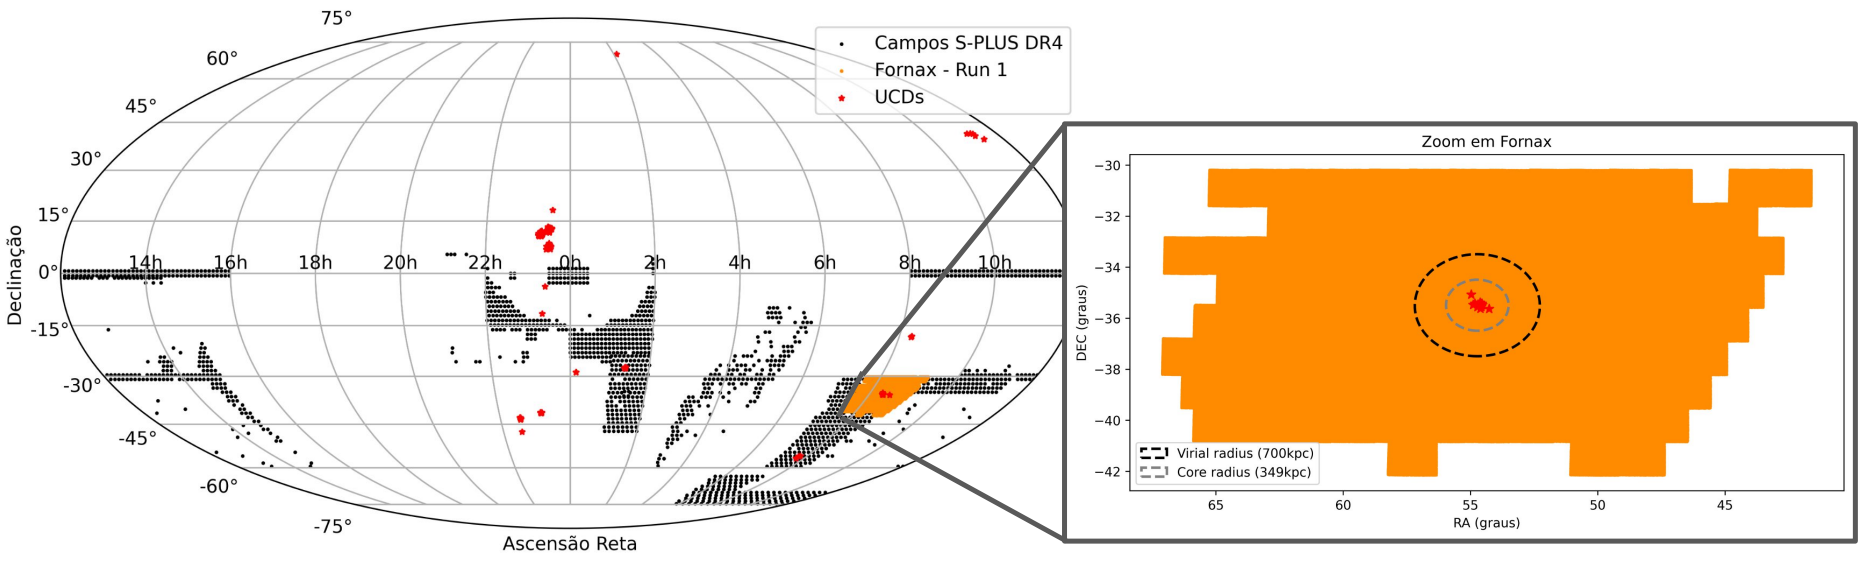
\includegraphics[width=0.7\columnwidth,angle=0]{distribution_know_ucds.png}
    \caption[]{Distribuição dos campos observados do S-PLUS DR4 no céu em coordenadas equatoriais. Os pontos pretos representam os campos do S-PLUS DR4, enquanto os pontos azuis indicam as UCDs selecionadas como conhecidas vindas de \cite{catalog_ucds}. A área em laranja corresponde aos do Aglomerado de Fornax com a redução da fotometria vindas de \cite{haack2024splusfornaxprojectsfp}, denominado \textit{Run 1}. As linhas de grade mostram a Ascensão Reta (em horas) e Declinação (em graus).}
    \label{distribution_know_ucds}
\end{figure}

\vspace{\baselineskip}

Os objetos compilados presentes na nossa amostra de Fornax, tiveram as propriedades estudadas por \cite{Mieske_2008_2}, em que todos os alvos foram confirmados como pertencentes ao cluster por meio de pesquisas espectroscópicas (\citealt{Drinkwater_2000}, \citealt{Mieske_2002} \& \citeyear{Mieske_2004}, \citealt{Richtler_2004} \& \citeyear{Richtler_2008}). Dessas descobertas, as 5 primeiros UCDs (chamadas de UCDs clássicas) foram encontrados em Fornax, e que são a confirmação vinda de \cite{Drinkwater_2000}.

\vspace{\baselineskip}

Dessas UCD conhecidas, foi feito um cruzamento com os dados de Fornax utilizado nesse trabalho. Deles tivemos 16 objetos correspondentes na nossa amostra. Na Tabela \ref{ucds_fornax_propriedades} temos a lista dessas UCDs conhecidas e suas propriedades fornecidas de \citealt{Mieske_2008_2}.

\begin{table}[!ht]
    \centering
    \caption{Propriedades dos UCDs identificados na região de Fornax com dados na amostra deste estudo, fornecidas de \citealt{Mieske_2008_2}.}
    \begin{tabular}{lcccccccc}
        \toprule
        Nome & RA & Dec & Massa & $M/L$ & [Fe/H] & $r_h$ & $\sigma$ \\
        & (graus) & (graus) & ($10^6 \, M_\odot$) & & (dex) & (pc) & (km/s)\\
        \midrule
        UCD3, F-19 & 54.72542 & -35.55933 & $93.6 \pm 14.0$ & $4.69 \pm 0.70$ & -0.4 & 89.7 & 22.8 \\
        UCD1       & 54.26375 & -35.63461 & $32.1 \pm 3.9$  & $4.99 \pm 0.60$ & -0.7 & 22.4 & 27.1 \\
        F-24       & 54.89958 & -35.47350 & $24.5 \pm 7.8$  & $3.44 \pm 1.10$ & -0.4 & 29.5 & 21.4 \\
        UCD5       & 54.96908 & -35.07336 & $18.0 \pm 4.5$  & $3.37 \pm 0.85$ & -1.2 & 31.2 & 18.7 \\
        F-1a       & 54.52625 & -35.48300 & $16.2 \pm 3.8$  & $2.45 \pm 0.58$ & 0.0  & 23.1 & 18.7 \\
        F-9        & 54.60625 & -35.62853 & $14.1 \pm 3.6$  & $4.72 \pm 1.20$ & -0.8 & 9.1  & 25.7 \\
        F-5        & 54.54500 & -35.42950 & $13.7 \pm 2.4$  & $3.16 \pm 0.55$ & -0.3 & 5.0  & 34.5 \\
        F-6        & 54.56875 & -35.43878 & $12.5 \pm 2.4$  & $5.32 \pm 1.00$ & 0.2  & 7.3  & 27.3 \\
        F-7        & 54.57333 & -35.55067 & $10.5 \pm 1.4$  & $4.21 \pm 0.57$ & -1.3 & 14.9 & 20.1 \\
        F-12       & 54.62083 & -35.38231 & $8.3 \pm 2.9$   & $2.36 \pm 0.83$ & -0.4 & 10.3 & 22.9 \\
        F-11       & 54.61792 & -35.42736 & $5.7 \pm 3.7$   & $1.64 \pm 1.10$ & -0.9 & 3.6  & 26.2 \\
        F-34       & 54.55292 & -35.48250 & $5.5 \pm 1.3$   & $3.17 \pm 0.74$ & -0.9 & 4.0  & 24.6 \\
        F-22       & 54.82375 & -35.42503 & $5.3 \pm 1.0$   & $2.13 \pm 0.39$ & -0.4 & 10.0 & 22.8 \\
        F-53       & 54.66917 & -35.48611 & $3.9 \pm 1.0$   & $2.66 \pm 0.69$ & -0.9 & 4.4  & 19.6 \\
        F-51       & 54.57125 & -35.44203 & $3.5 \pm 0.9$   & $2.38 \pm 0.62$ & -0.8 & 4.2  & 20.1 \\
        F-59       & 54.70375 & -35.46225 & $1.3 \pm 0.6$   & $0.94 \pm 0.43$ & -2.1 & 5.7  & 9.8  \\
        \bottomrule
    \end{tabular}
    \label{ucds_fornax_propriedades}
\end{table}

Fazendo um cruzamentos das UCDs conhecidas do catálogo \cite{catalog_ucds} com os dados da fotometria do S-PLUS DR4 originais, tivemos 9 dos objetos, em comparação com os 16 que obtemos anteriormente. Isso é, ressaltamos aqui como a redução da fotometria de Fornax vindas de \cite{haack2024splusfornaxprojectsfp} é importante para identificação das nossas galáxias de interesse.

\vspace{\baselineskip}

Fazendo um cruzamento dessas UCDs conhecidas nos nossos dados com o catálogo GAIA DR3 (\cite{GAIA_DR3}), que fornece informações de classificação estrela-galáxia-quasar, observamos que das 16, 8 têm probabilidade maior que 50\% de serem galáxias e 8 têm probabilidade maior que 50\% de serem estrelas. Esse fato mostra a dificuldade de classificação desses objetos, mesmo levando em conta a morfologia e movimento próprio desses objetos levados em consideração pelo GAIA. Mostramos na Tabela \ref{tab_ucds_stars_galaxy_like} as médias e desvios padrões das magnitudes dos dados usados desses dois grupos.

\begin{table}[!ht]
    \centering
    \caption{Comparação das 12 magnitudes do S-PLUS DR4 (Run 1) da abertura PETRO corrigidas pela extinção entre as UCDs conhecidas, separadas em dois grupos: classificação estrela (PSS > 0.5) ou galáxia (PGal > 0.5) pelo Gaia DR3.}   \begin{tabular}{lcccc}
        \toprule
        Filtro & \multicolumn{2}{c}{UCD - Galáxia} & \multicolumn{2}{c}{UCD - Estrela} \\
        & Média & $\sigma$ & Média & $\sigma$ \\
        \midrule
        F378 & 21,67 & 0,96 & 21,75 & 0,39 \\
        F378 & 21,03 & 0,97 & 21,83 & 0,67 \\
        F395 & 21,53 & 2,01 & 21,36 & 0,65 \\
        F410 & 20,06 & 0,67 & 21,53 & 0,53 \\
        F430 & 20,12 & 0,84 & 21,19 & 0,56 \\
        g    & 19,65 & 0,77 & 21,03 & 0,64 \\
        F515 & 19,36 & 0,75 & 20,60 & 0,67 \\
        r    & 18,95 & 0,71 & 20,35 & 0,41 \\
        F660 & 18,86 & 0,72 & 20,24 & 0,37 \\
        i    & 18,63 & 0,78 & 20,14 & 0,56 \\
        F861 & 18,47 & 0,78 & 19,84 & 0,42 \\
        z    & 18,39 & 0,80 & 19,97 & 0,49 \\
        \bottomrule
    \end{tabular}
    \label{tab_ucds_stars_galaxy_like}
\end{table}

\vspace{\baselineskip}

Concluímos pela Tabela \ref{tab_ucds_stars_galaxy_like} que o grupo de UCDs classificados como galáxias pelo GAIA DR3 é mais brilhante que o grupo classificado como estrelas. Observando ainda o banda fotométrica $r$, usada como referência devido sua profundidade e qualidade, temos as UCDs classificadas como galáxias no intervalo de 17,5 a 19,7 magnitudes, enquanto as classificadas como estrelas estão no intervalo de 19,5 a 20,8 magnitudes. Com esses intervalos, podemos usar de referência para a seleção dos objetos de interesse.

\vspace{\baselineskip}

Pela propriedades da Tabela \ref{ucds_fornax_propriedades}, mostramos na Figura \ref{r_h_M_ucds} a relação entre a massa e o raio de meia luz das UCDs conhecidas de Fornax. Observamos uma conclusão similar, que o grupo de UCDs classificados como galáxias pelo GAIA DR3 é mais brilhante que o grupo classificado como estrelas, e assim, tendo uma relação entre a massa e o raio de meia luz maior.


\begin{figure}[!ht]
    \centering
    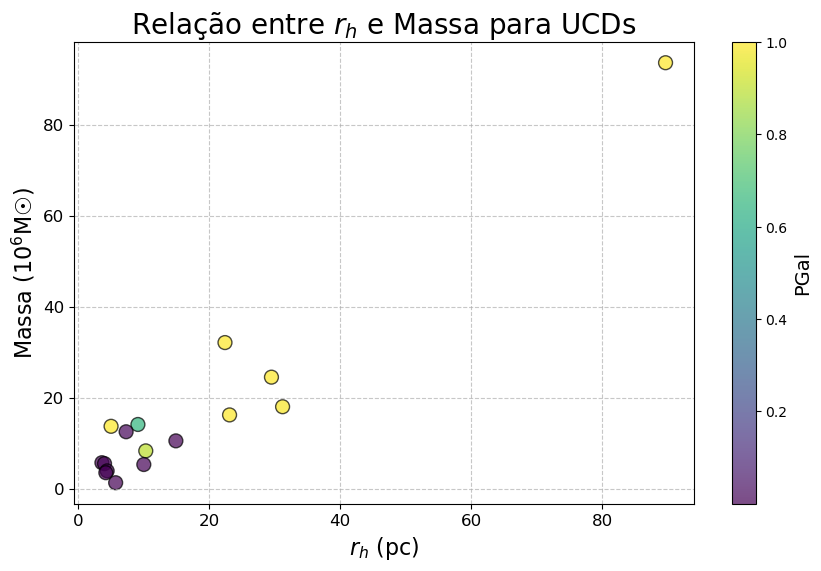
\includegraphics[width=0.6\columnwidth,angle=0]{r_h_M_ucds.png}
    \caption[]{Relação entre a massa e o raio de meia luz das UCDs conhecidas de Fornax. Classificação estrela (PSS > 0.5) ou galáxia (PGal > 0.5) pelo Gaia DR3.}
    \label{r_h_M_ucds}
\end{figure}



\section{Amostra de treino}
Para a amostra de treino, é desejável implementar uma estratégia que auxilie na identificação de candidatas a UCDs. Uma abordagem comum é a utilização de um classificador, onde um modelo é treinado com um conjunto de dados rotulados e, posteriormente, é capaz de classificar novos objetos com base nas características aprendidas durante o treinamento.

\vspace{\baselineskip}

Um exemplo parecido é o problema de classificação de quasares, que são fontes pontuais facilmente confundidas com estrelas, mas possuem características que os distinguem como galáxias. Nesse caso, um modelo de classificação pode ser feito treinando com dados de quasares e estrelas, realizando a separação deles. Porém, para UCDs, temos uma quantidade limitada de objetos conhecidos, impossibilitando um conjunto de dados grande o suficiente para treinar um modelo de classificação direto de UCDs.

\vspace{\baselineskip}

A proposta nesse trabalho é utilizar um modelo de classificação indireta, onde treinamos um modelo para classificar objetos em duas classes: objetos compactos e objetos extensos. Um dos parâmetros disponíveis para os objetos da amostra é a largura à meia altura, full width at half maximum (\textit{FWHM}). O \textit{FWHM} representa a largura do perfil de intensidade de uma fonte de luz na metade de sua intensidade máxima. Em nosso estudo, essa métrica é particularmente relevante, pois ao lidar com estrelas e UCDs, ela auxilia na identificação de fontes pontuais. Para cada uma das 12 bandas fotométricas, temos a \textit{FWHM} disponível associado. 

As estrelas, por sua natureza, são fontes pontuais; por isso, esperamos que a \textit{FWHM} desses objetos seja menor do que a de objetos extensos, como as galáxias, exceto, claro, para galáxias ultra compactas.

\vspace{\baselineskip}

Realizamos um cruzamento de dados de treinamento com o catálogo GAIA DR3 (\cite{GAIA_DR3}), que fornece informações de classificação estrela-galáxia-quasar. Com esses dados, selecionamos um subconjunto de objetos com as probabilidades de serem estrelas e galáxias maiores que 90\%. A partir desse subconjunto, analisa-se a distribuição dos valores de \textit{FWHM} para estrelas e galáxias em cada banda fotométrica. Na Figura \ref{distribution_of_stars_and_galaxies}, temos um histograma da distribuição de \textit{FWHM} para estrelas e galáxias da banda $r$, sendo ela a banda com a melhor separação entre as duas classes.

\begin{figure}[!ht]
    \centering
    \begin{minipage}{0.45\textwidth}
        \centering
        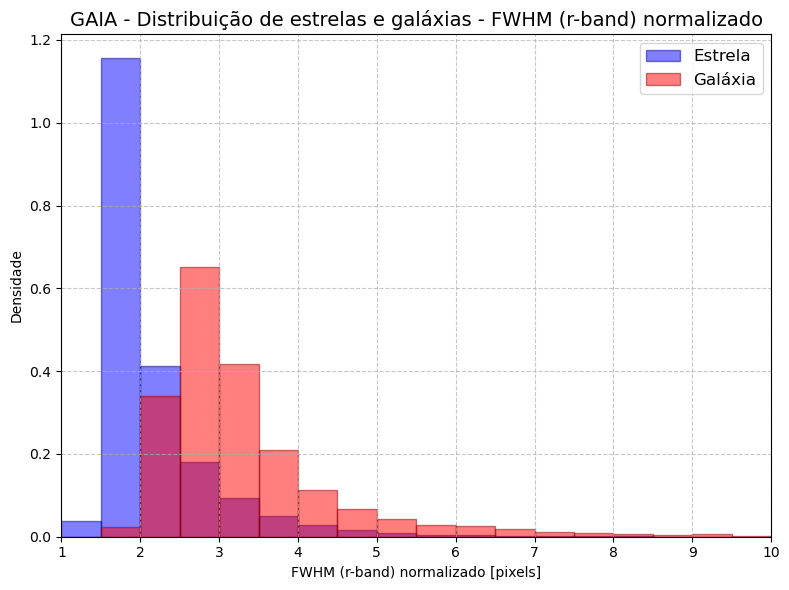
\includegraphics[width=\linewidth]{distribution_of_stars_and_galaxies.png}
        \caption{Histograma da distribuição de \textit{FWHM (r-band)} dos objetos do cruzamento do S-PLUS DR4 de Fornax, com o catálogo GAIA DR3 com a classificação para estrelas e galáxias com probabilidade maior que 90\%.}
        \label{distribution_of_stars_and_galaxies}
    \end{minipage}\hfill
    \begin{minipage}{0.45\textwidth}
        \centering
        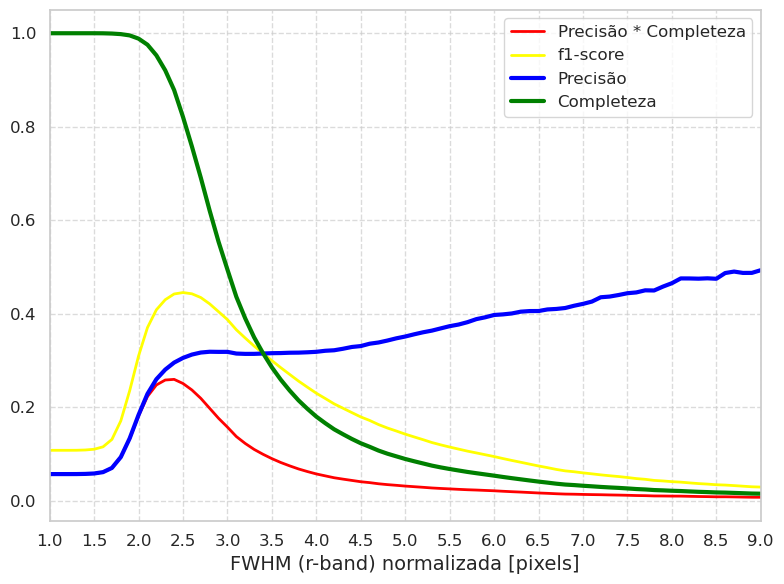
\includegraphics[width=\linewidth]{purity_completeness.png}
        \caption{Relação entre Pureza e Completeza para diferentes cortes de \textit{FWHM}. O ponto ideal é aquele que maximiza o produto entre as duas variáveis, indicando o corte que melhor separa as duas classes.}
        \label{purity_completeness}
    \end{minipage}
\end{figure}

\vspace{\baselineskip}

Há uma diferença entre os picos das distribuições de \textit{FWHM} para estrelas e galáxias. Portanto, o objetivo é definir um corte na \textit{FWHM} para selecionar dois conjuntos: um contendo objetos compactos e outro, objetos extensos. No conjunto de objetos compactos, predominam as estrelas, enquanto no conjunto de objetos extensos, as galáxias são mais representativas.

\vspace{\baselineskip}

A hipótese é que o modelo aprenda a distinguir as propriedades fotométricas de estrelas e galáxias independentemente da morfologia (ou FWHM) do objeto; numa segunda etapa, procuramos entre os objetos com morfologia estelar, aqueles cuja fotometria indica que têm alta probabilidade de serem galáxias

% A hipótese é que, ao treinar um modelo de classificação usando as magnitudes e cores, o modelo será capaz de aprender a distinguir entre as duas classes propostas. A busca por candidatas a UCDs pode ser feita a partir da seleção de objetos compactos (com valores de \textit{FWHM} menores) que são classificados como objetos extensos pelo modelo, ou seja, que possuem características fotométricas de galáxias.

\vspace{\baselineskip}

Para identificar, na Figura \ref{distribution_of_stars_and_galaxies}, a melhor divisão entre as duas classes, estabelecemos alguns cortes visando encontrar aquele que melhor separa cada população, minimizando a contaminação da população adjacente. Para cada corte, definimos duas variáveis: Pureza e Completeza, ambas com respeito às galáxias. A Pureza representa a fração de galáxias após o corte em relação ao total de objetos restantes no corte final, fornecendo uma medida da pureza das galáxias no subconjunto.

Por outro lado, a Completeza representa a fração de galáxias após o corte em relação ao número total de galáxias que existiam, fornecendo uma estimativa de quantas galáxias são perdidas durante a seleção.

A Figura \ref{purity_completeness} ilustra a relação entre Pureza e Completeza para diferentes valores de corte de \textit{FWHM}. O ponto ótimo que adotamos é aquele que maximiza o produto dessas duas variáveis, representando o corte que proporciona a melhor separação entre as duas classes.

\vspace{\baselineskip}

Os valores selecionados para o corte ficaram com um \textit{FWHM (r-band)} de 3.5 pixels. Esse corte corresponde ao ponto para a maximização do limite das classes de seleção de galáxias, associada como sendo a classe de extensos. Porém, os objetos que estão abaixo desse corte não são apenas estrelas, e para evitar a sua confusão, realizamos um corte para objetos compactos com \textit{FWHM} menores que 3 pixels, em que tivemos melhores resultados nos classificadores iniciais testados. Assim, para a amostra de treino, selecionamos objetos com \textit{FWHM} (r-band) menores que 3 pixels como compactos e objetos com \textit{FWHM (r-band)} maiores que 3.5 pixels como extensos.

\vspace{\baselineskip}

Na Figura \ref{distribuicao_fwhm_image_r_r_petro_ucds_fornax} mostramos a distribuição de \textit{FWHM (r-band)} em função da banda \textit{r\_PETRO} para UCDs de Fornax. Percebemos uma certa tendência, onde para as UCDs mais brilhantes temos um \textit{FWHM (r-band)} maior, porém sem uma quantidade significativa de objetos não podemos afirmar com certeza essa relação.

\begin{figure}[!ht]
    \centering
    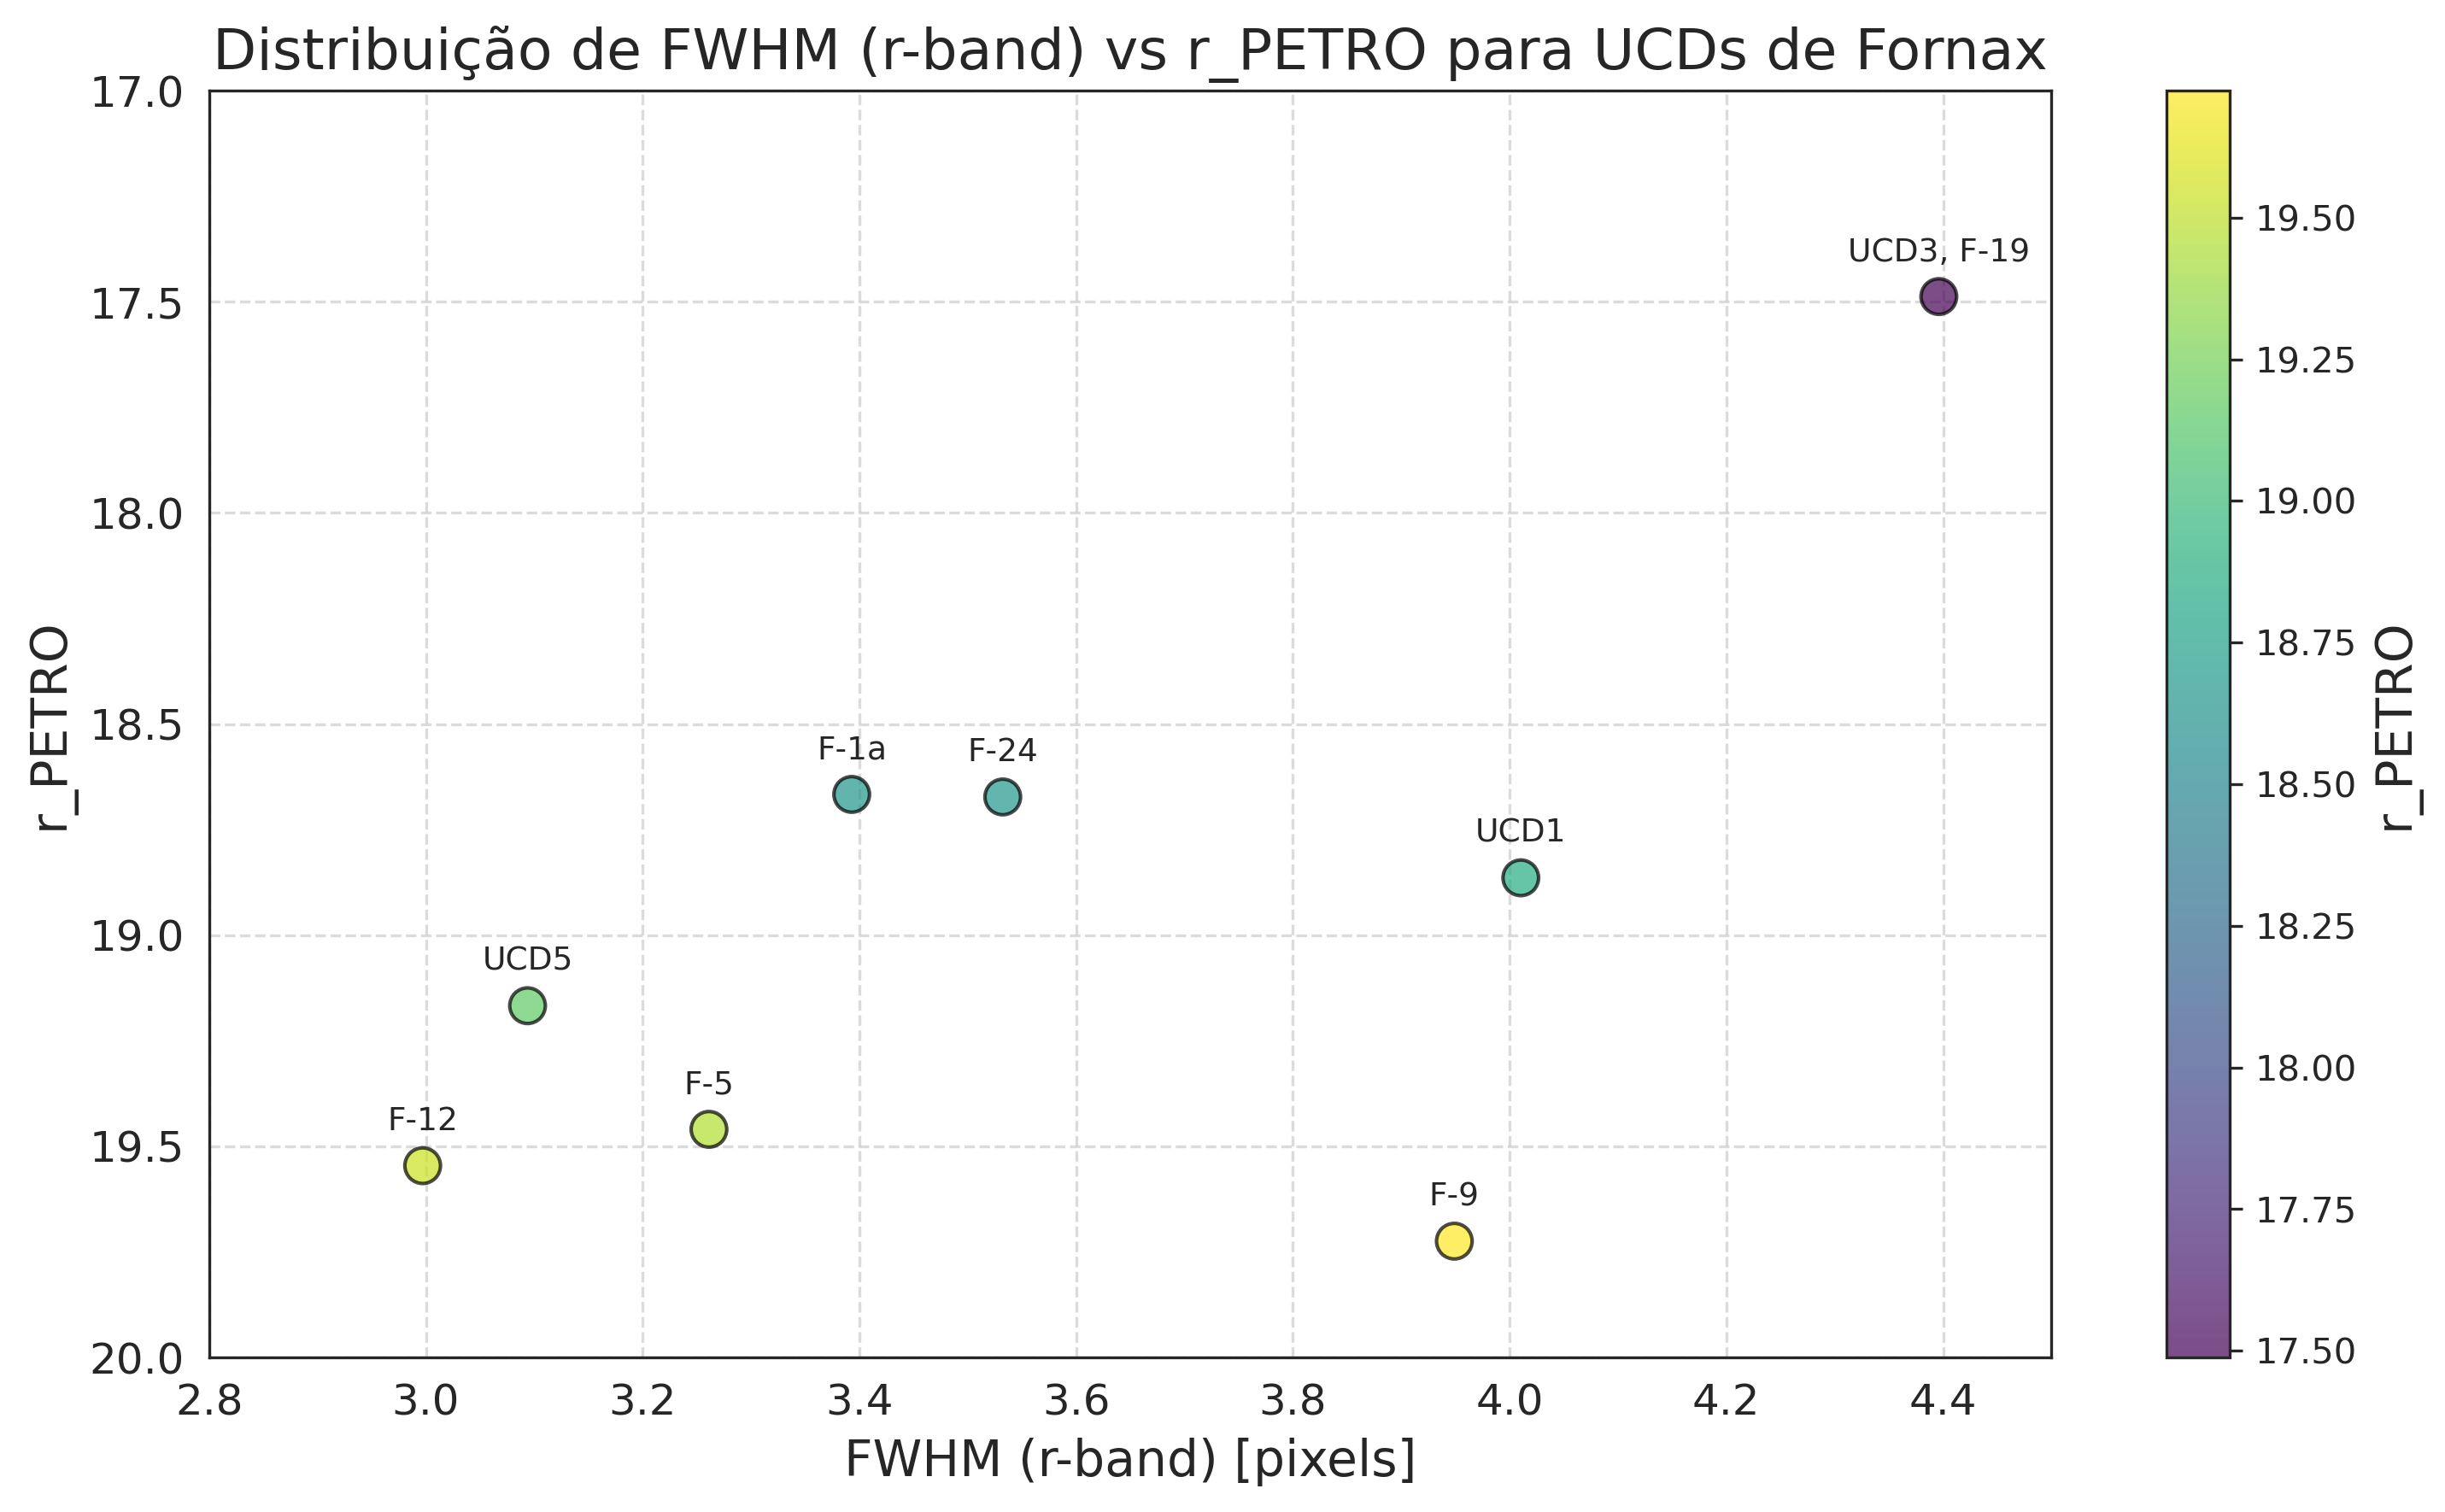
\includegraphics[width=0.8\columnwidth,angle=0]{distribuicao_fwhm_image_r_r_petro_ucds_fornax.png}
    \caption[]{Distribuição de \textit{FWHM (r-band)} em função da banda \textit{r\_PETRO} para UCDs de Fornax.}
    \label{distribuicao_fwhm_image_r_r_petro_ucds_fornax}
\end{figure}

\vspace{\baselineskip}

Foram feitos também cortes na magnitude \textit{g\_PETRO}$\geq$13, evitando objetos mais brilhantes e saturados. Cortamos também \textit{g\_PETRO}$\leq$21, para evitar a contaminação de aglomerados globulares. Cortamos nas 12 magnitudes da abertura PETRO em magnitudes maiores do que 30, evitando objetos com baixa qualidade de medição, com erros fotométricos altos. Cortamos também em cada uma das mesmas bandas valores de \textit{flag0}$\leq$2, que são objetos com problemas de qualidade de medição.

\vspace{\baselineskip}

Na Figura \ref{amostra_treino}, temos a magnitude \textit{g\_PETRO} em função da \textit{FWHM (r-band)} para a divisão entre as duas classes adotadas.

\begin{figure}[!ht]
    \centering
    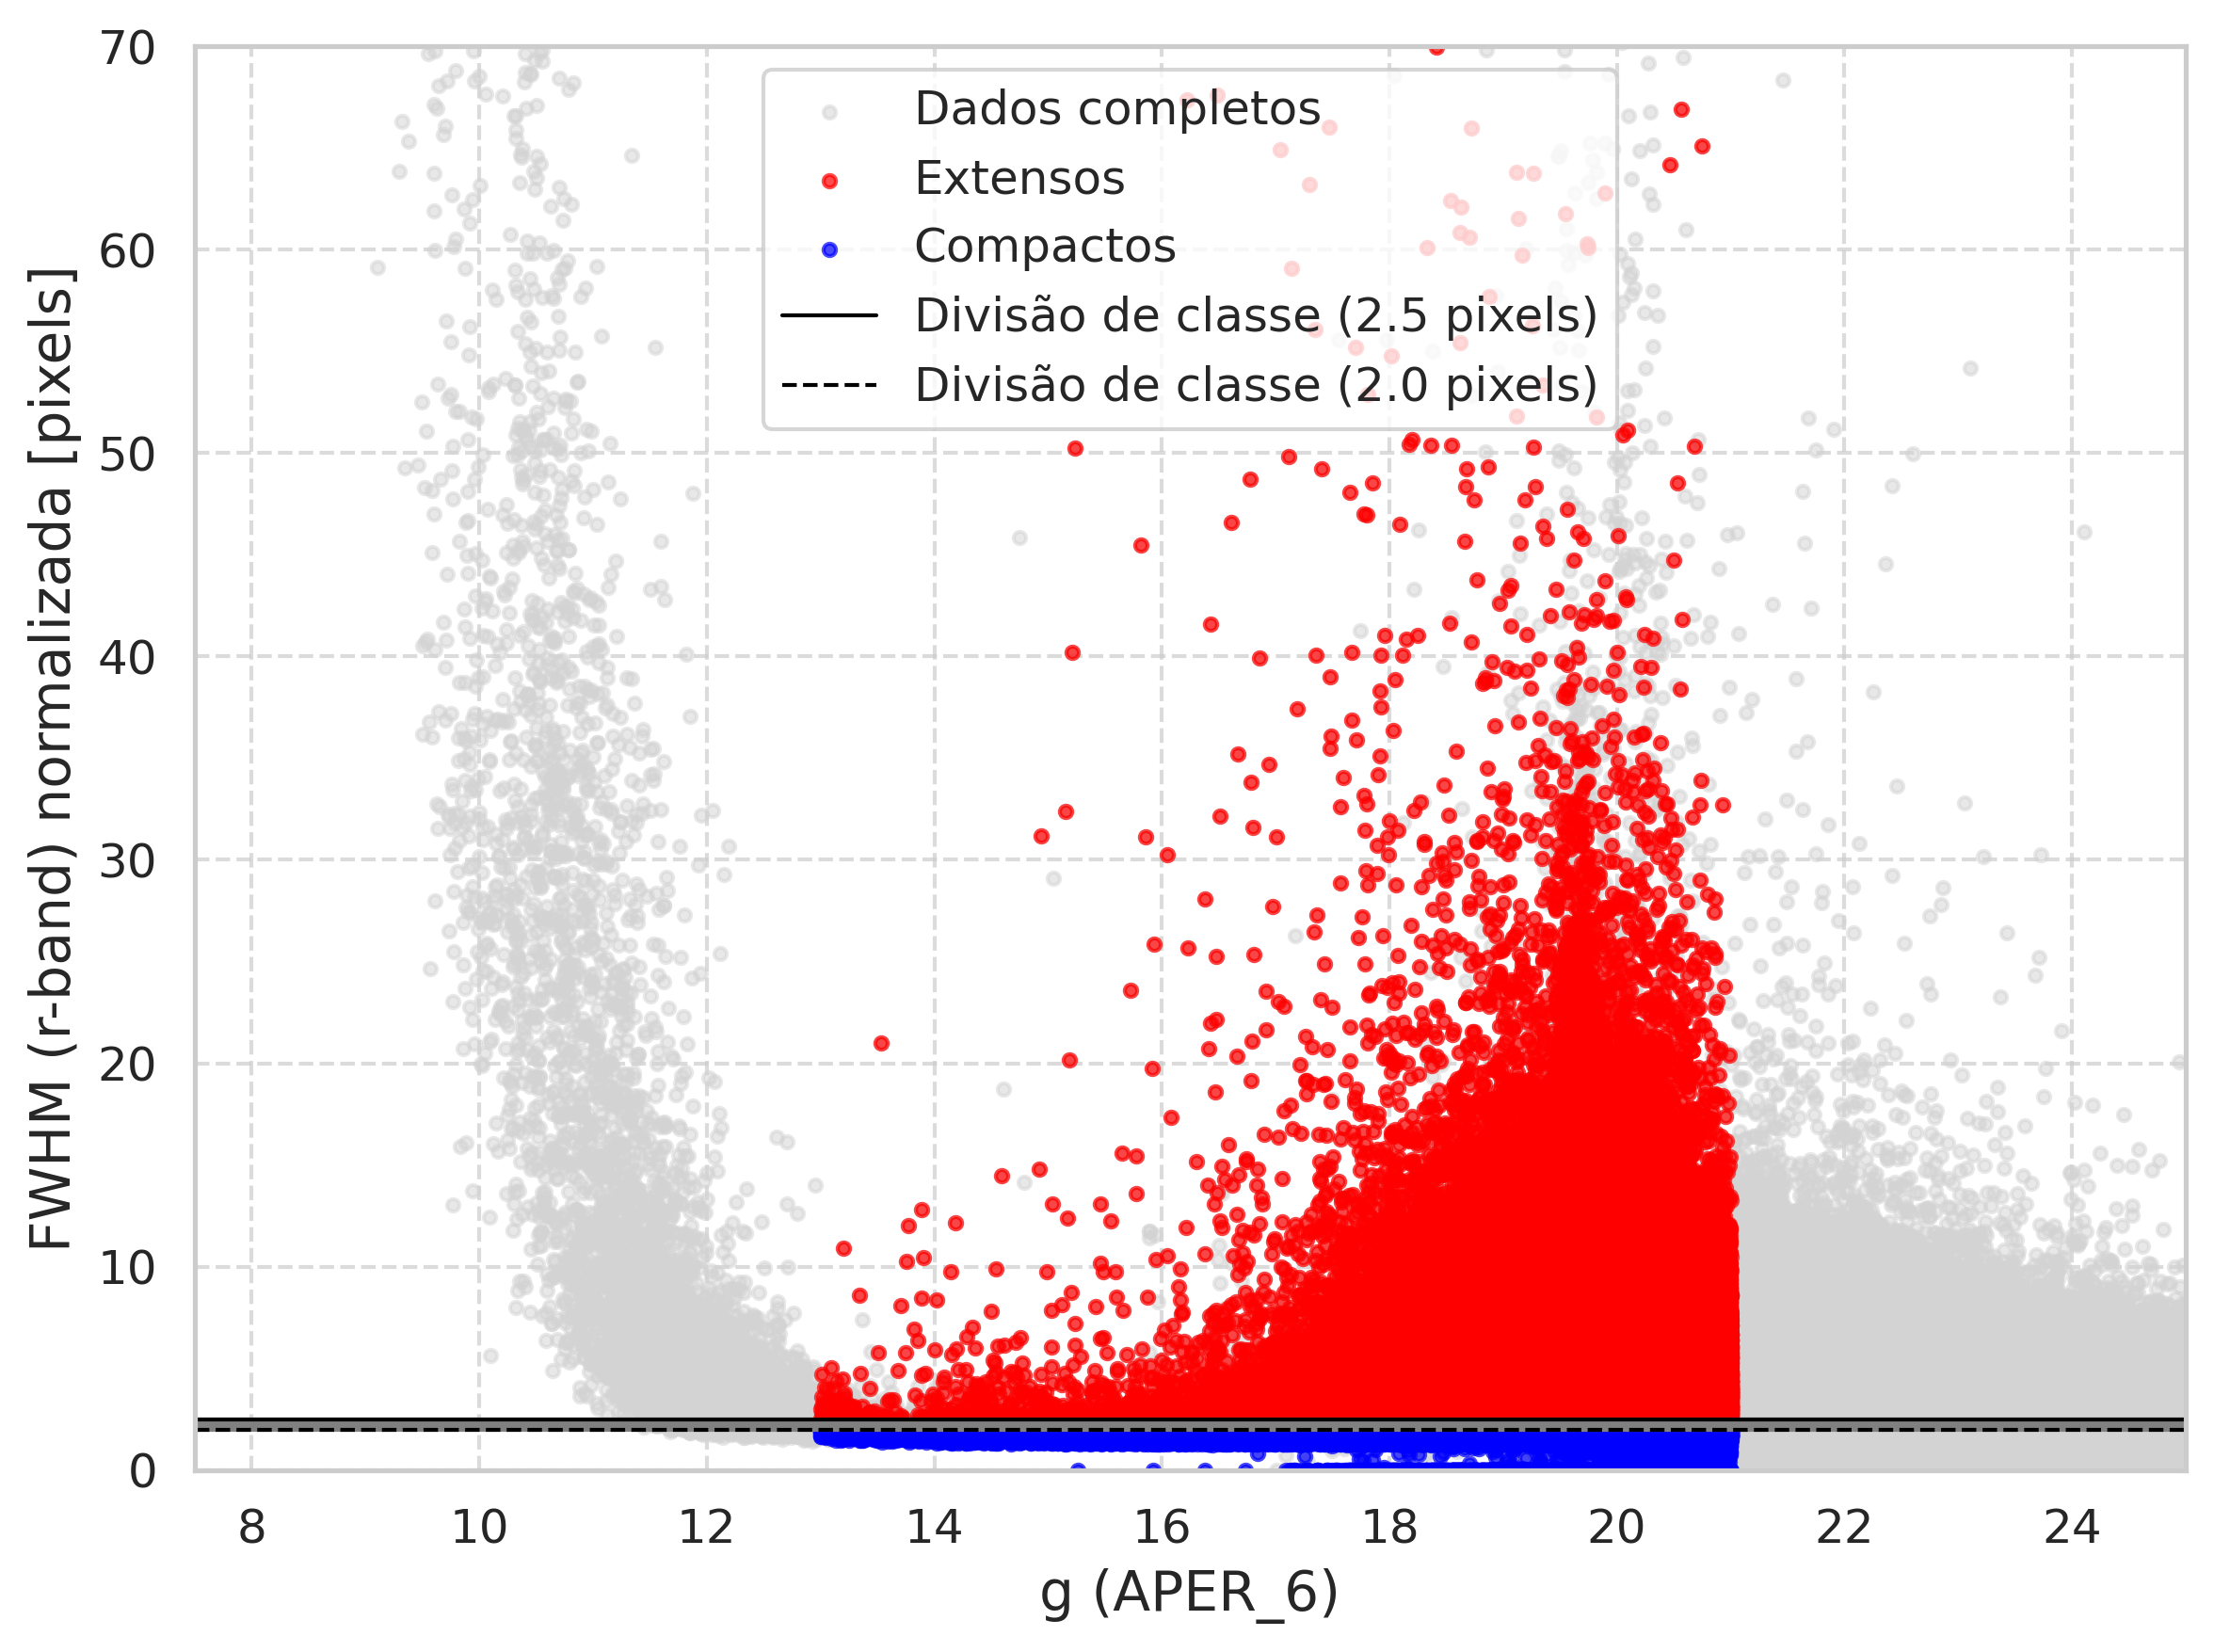
\includegraphics[width=0.75\columnwidth,angle=0]{amostra_treino.png}
    \caption[]{Distribuição da Largura Total na Metade Máxima (\textit{FWHM} r-band) em função da magnitude \textit{g\_PETRO} para objetos na região de Fornax, usando dados do S-PLUS Data Release 4. Objetos compactos são representados por pontos azuis, enquanto objetos extensos são indicados por pontos vermelhos. Os dados totais são mostrados em cinza. Divisão das classes: compactos (\textit{FWHM}$\leq$3 pixels) e extensos (\textit{FWHM}$\geq$3.5 pixels).}
    \label{amostra_treino}
\end{figure}

\vspace{\baselineskip}

\section{Valores faltantes na amostra de treino}
Ao preparar os dados para treinar modelos com medições do S-PLUS, foi identificado que algumas colunas apresentam valores faltantes para determinados objetos em uma ou mais das 12 bandas fotométricas. 

Na Figura \ref{missing_values_hist} temos um gráfico da distribuição da quantidade de dados para cada um dos atributos do conjunto de magnitudes.

\begin{figure}[!ht]
    \begin{center}
    % \setcaptionmargin{1cm}
    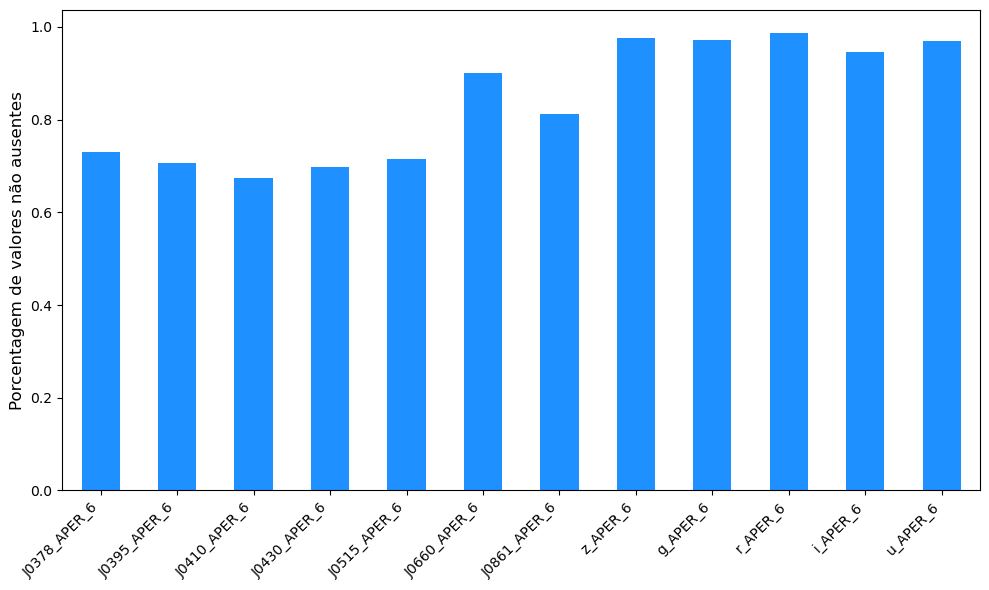
\includegraphics[width=0.76\columnwidth,angle=0]{missing_values_hist.png}
    \caption[]{Distribuição de valores em cada banda fotométrica. Cada barra representa a quantidade de objetos com valores disponíveis para a respectiva banda.}
    \label{missing_values_hist}
    \end{center}
\end{figure}

\vspace{\baselineskip}

O gráfico mostra que a quantidade de dados ausentes varia consideravelmente entre as diferentes bandas fotométricas. A banda $u$, juntamente com algumas estreitas como $J0378$, $J0395$, $J0410$ e $J0430$, são as que apresentam a maior quantidade de valores faltantes que podem prejudicar a análise.

\vspace{\baselineskip}

Mostramos na Figura \ref{msno_matriz} uma outra visualização da distribuição dos dados faltantes, onde cada linha representa um objeto e cada coluna uma banda fotométrica. As células em branco indicam valores faltantes. A Figura \ref{msno_matriz_ord} mostra a mesma matriz, mas ordenada pela primeira coluna de atributos. Ordenamos a matriz para identificar padrões de valores faltantes que possam ser úteis para a imputação dos dados.

\begin{figure}[!ht]
    \centering
    \begin{minipage}{0.45\textwidth}
        \centering
        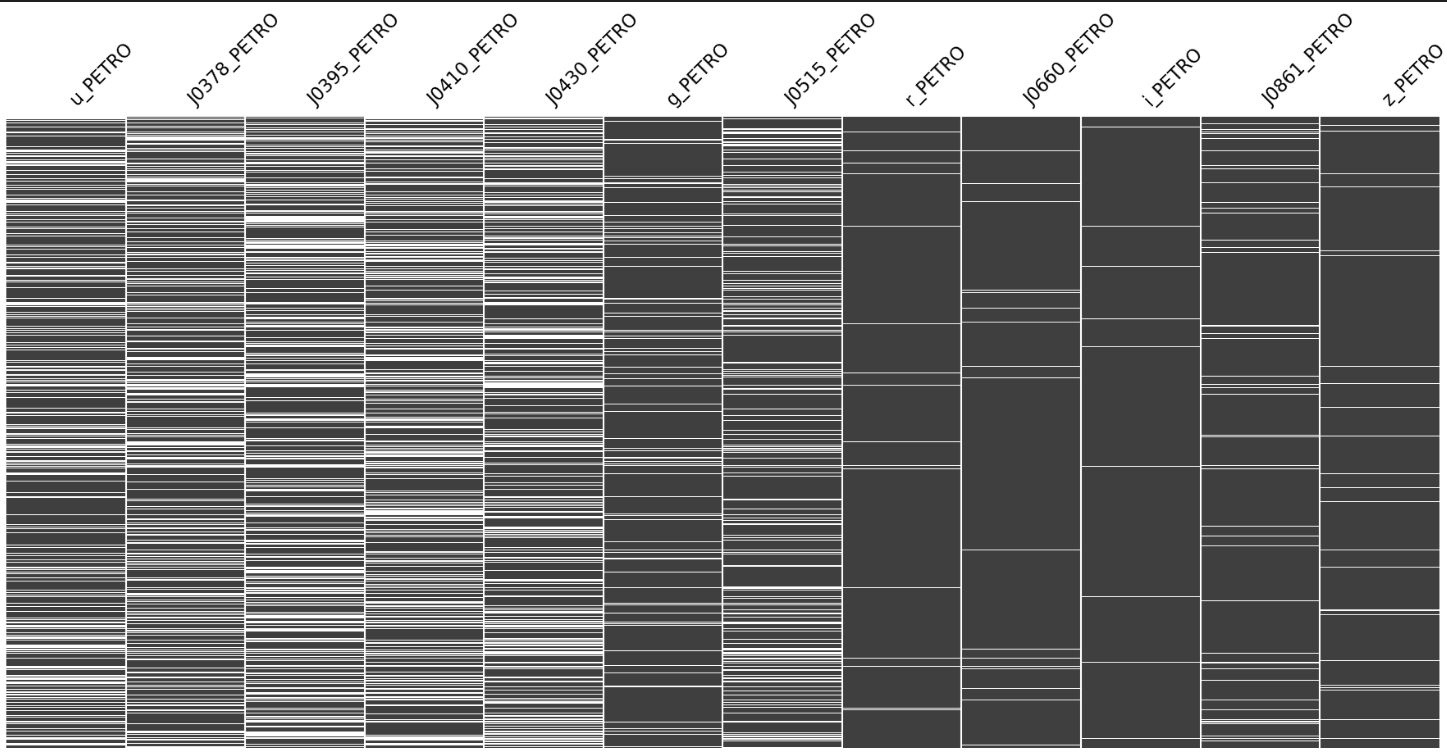
\includegraphics[width=\linewidth]{msno_matriz.png}
        \caption{Distribuição de valores em cada banda fotométrica. Cada barra representa a quantidade de objetos com valores disponíveis para a respectiva banda.}
        \label{msno_matriz}
    \end{minipage}\hfill
    \begin{minipage}{0.45\textwidth}
        \centering
        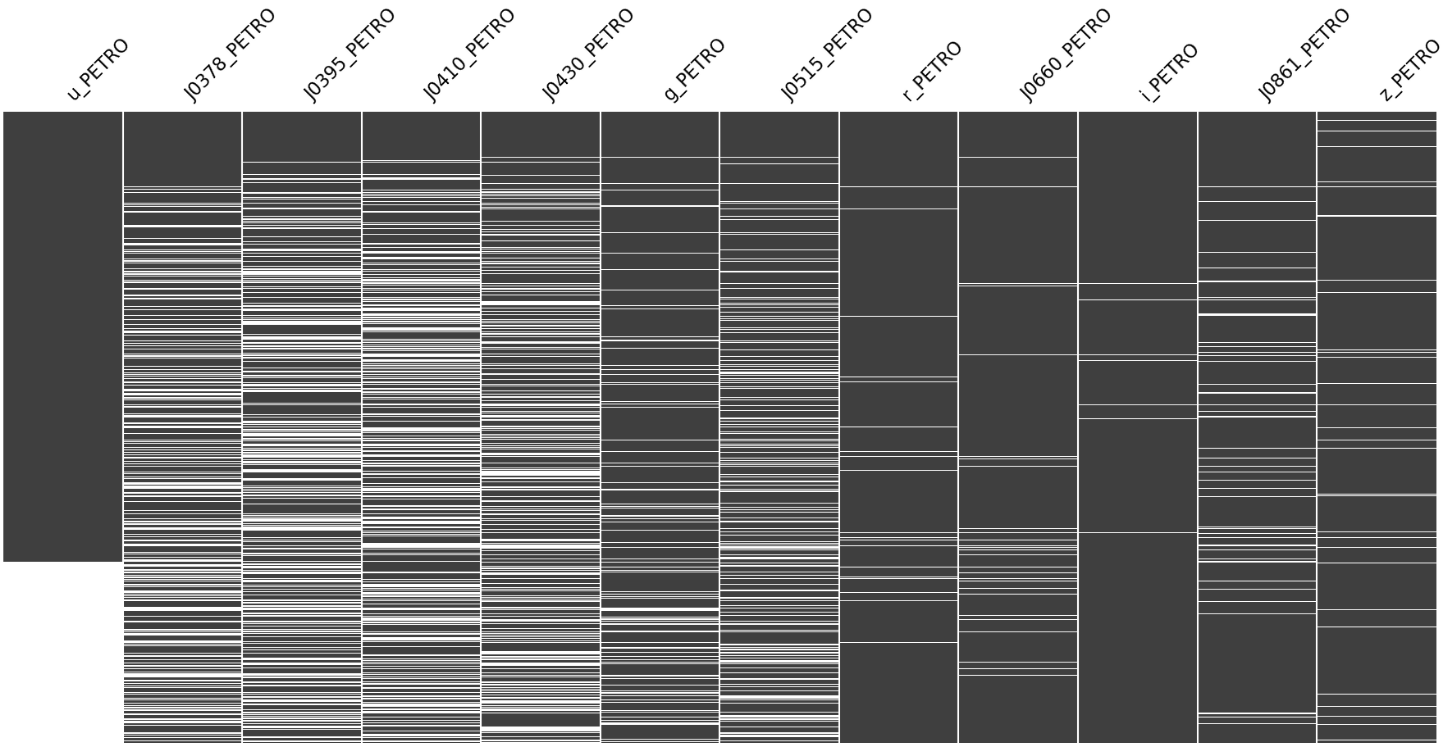
\includegraphics[width=\linewidth]{msno_matriz_ord.png}
        \caption{Distribuição de valores faltantes em cada banda fotométrica ordenada pela primeira coluna de atributos. Cada célula em branco indica um valor faltante.}
        \label{msno_matriz_ord}
    \end{minipage}
\end{figure}

\vspace{\baselineskip}

Um jeito melhor de visualizar se esses valores ausentes têm alguma correlação é vista na Figura \ref{matriz_correlacao}, que mostra a matriz de correlação entre os valores faltantes. Valores próximos de 1 ou -1 indicam que os valores faltantes estão, respectivamente, positivamente ou negativamente correlacionados. Valores próximos de 0 indicam que os valores faltantes são independentes.

\begin{figure}[!ht]
    \begin{center}
    % \setcaptionmargin{1cm}
    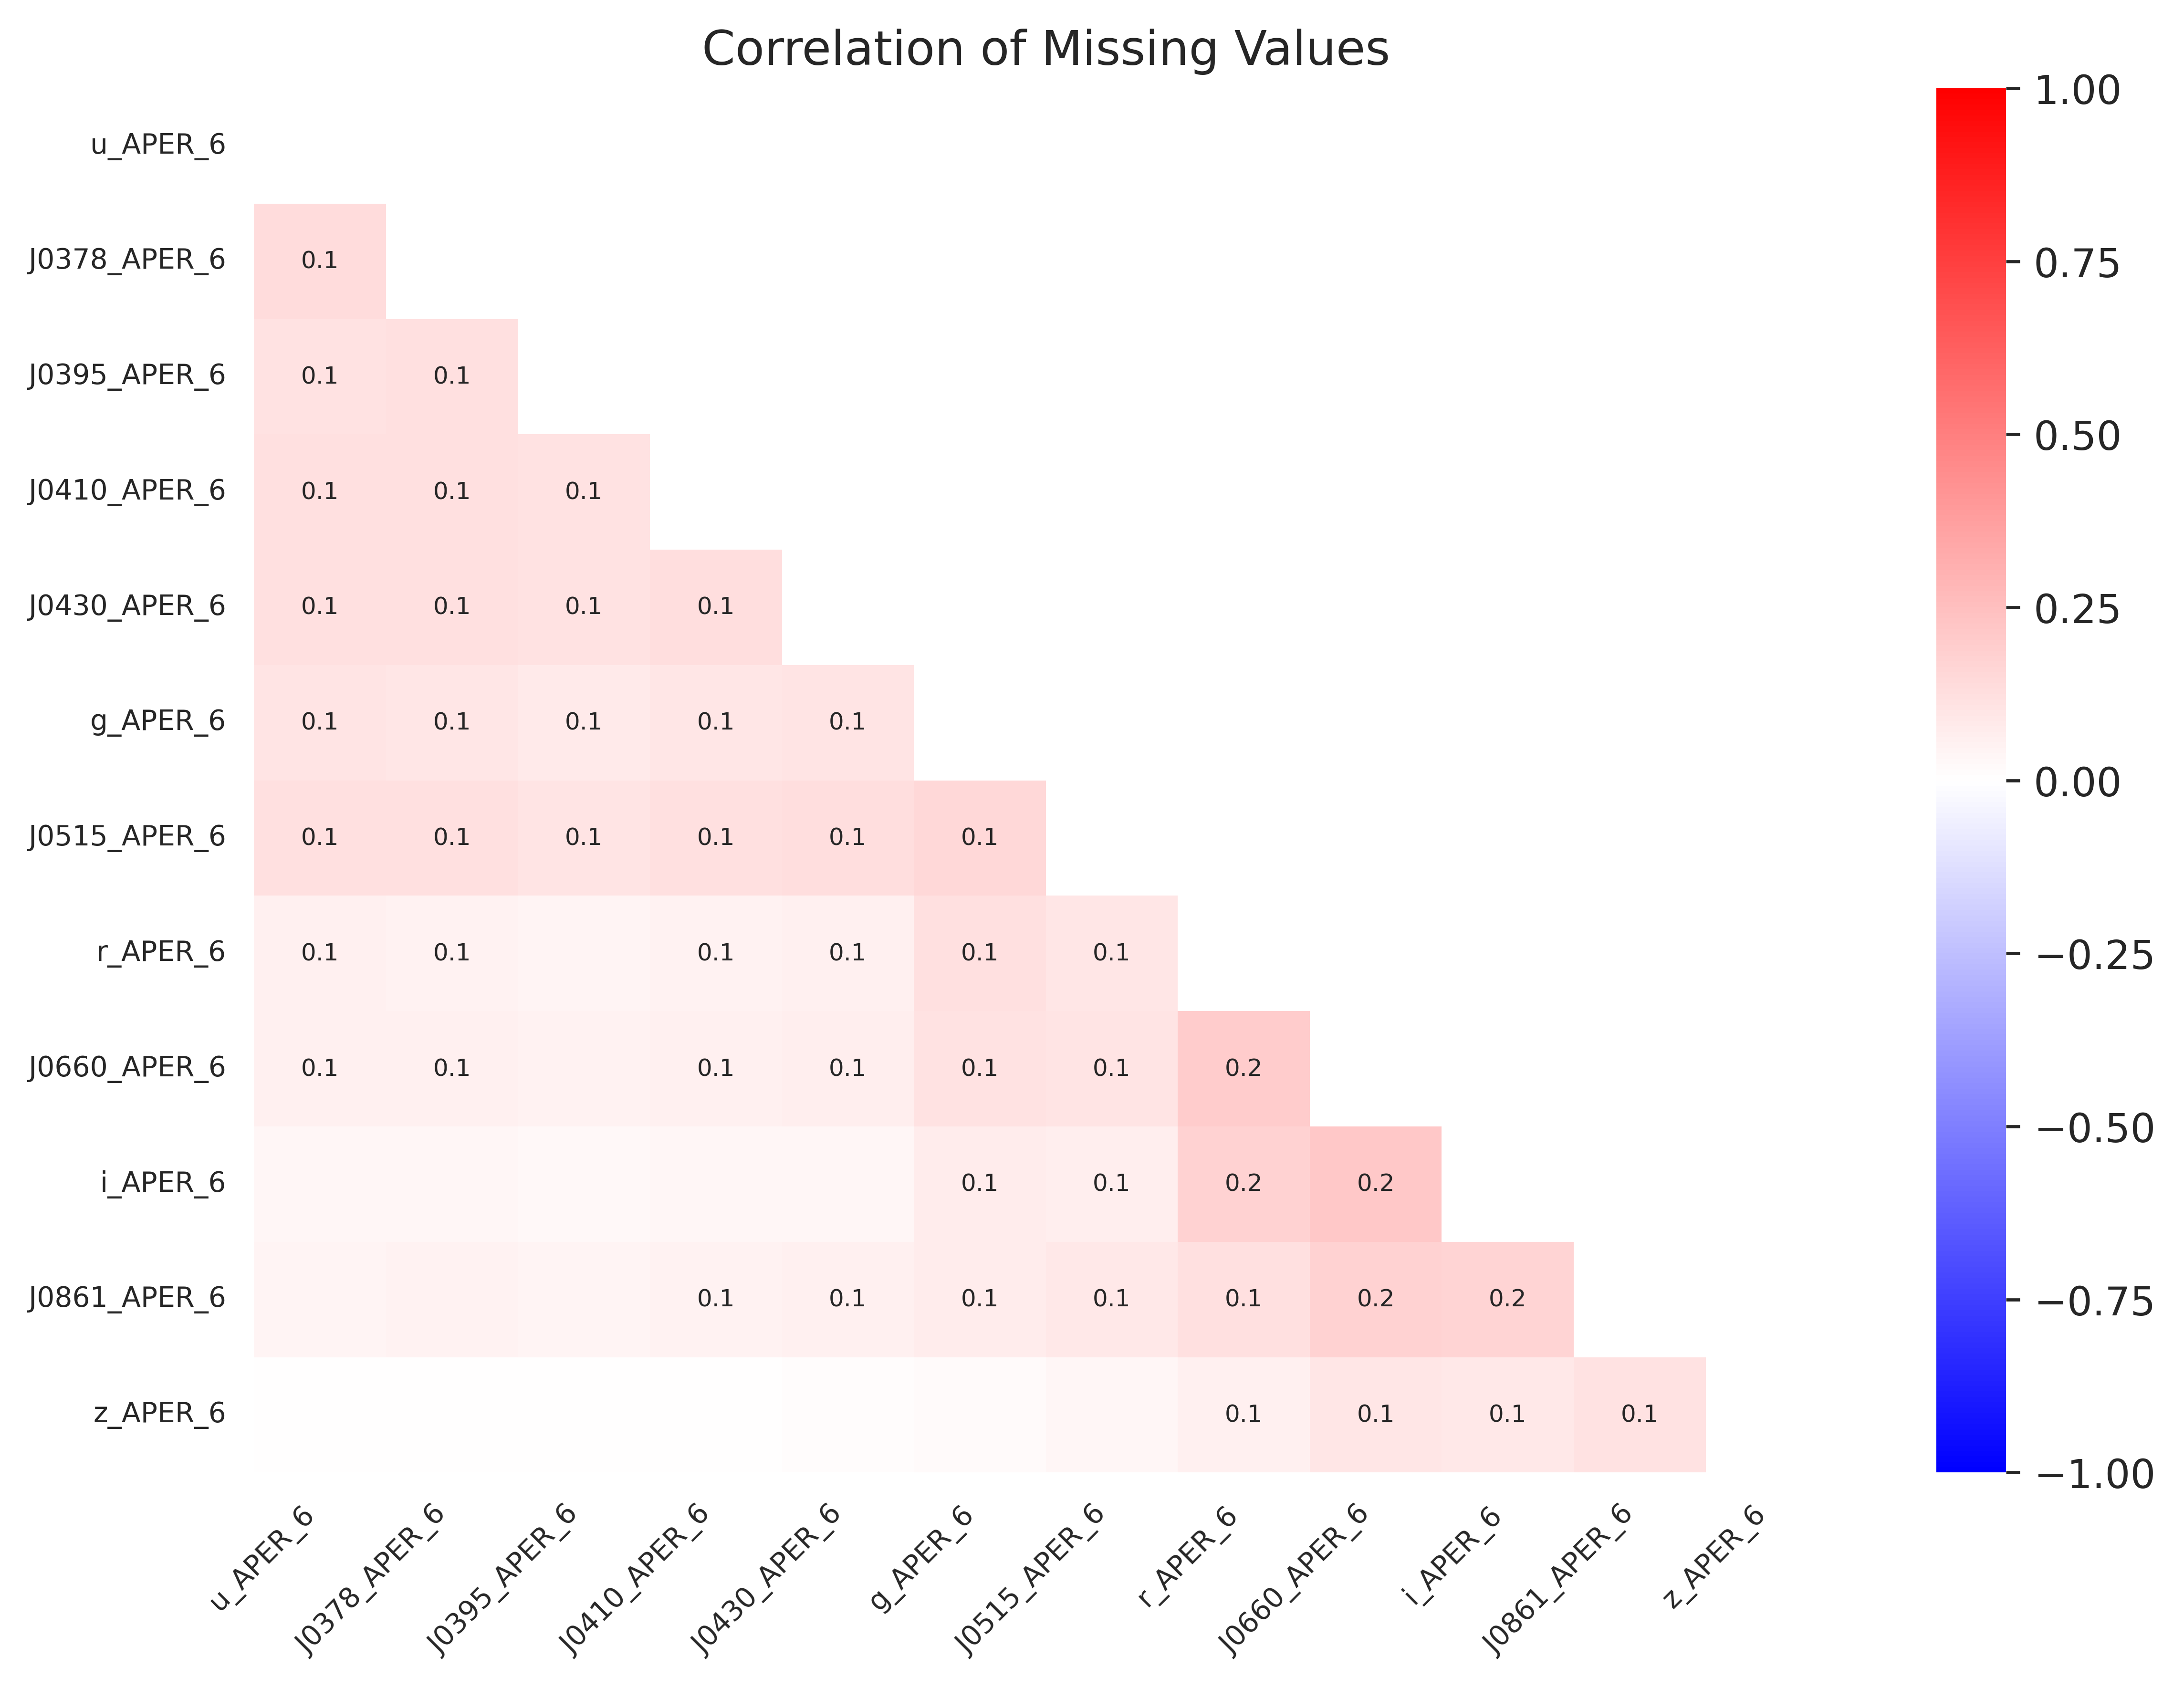
\includegraphics[width=0.85\columnwidth,angle=0]{matriz_correlacao.png}
    \caption[]{Matriz de correlação entre os valores faltantes. Cada célula contém o coeficiente de correlação entre os valores faltantes de duas bandas fotométricas.}
    \label{matriz_correlacao}
    \end{center}
\end{figure}

\vspace{\baselineskip}

Pela Figura \ref{matriz_correlacao}, observamos que a maioria dos valores faltantes não apresenta correlação significativa, sugerindo que os dados faltantes são independentes.

\vspace{\baselineskip}

Existem várias técnicas para lidar com esses valores ausentes. Um jeito fácil e comum é apenas remover os objetos que possuem algum dado faltante, mas isso pode gerar uma perda de informação para o treinamento. Outra alternativa é alterar os valores faltantes com a média dos valores restantes, mas com isso poderíamos introduzir um viés na nossa seleção. Há ainda a opção de utilizar algum valor padrão, como o uso \texttt{NaN} (Not a Number) ou -1, porém, essa estratégia pode acabar confundindo o classificador, principalmente se para o modelo esses valores não tiverem um significado claro.

\vspace{\baselineskip}

A técnica que adotamos para lidar com os valores faltantes foi a imputação dos dados utilizando o Método de Imputação Múltipla por Equações Encadeadas (MICE) (\citealp{MICE}). O MICE é um método de imputação que utiliza várias iterações de treinamento de modelos de aprendizado de máquina para prever os valores ausentes usando valores conhecidos de outras variáveis como preditores.

\section{Treinando o modelo}
Para treinar os modelos de classificação, utilizamos o algoritmo K-Nearest Neighbors (KNN). O KNN é um algoritmo de aprendizado supervisionado que classifica um objeto baseado em seus vizinhos mais próximos. Dada uma amostra de um conjunto de dados, ele irá calcular e avaliar as distâncias entre os objetos, e dada a classificação dos vizinhos mais próximos, o objeto será classificado de acordo.

\vspace{\baselineskip}

Para o treinamento do modelo, dividimos nossa amostra em duas classes: objetos compactos (classe 0) e objetos extensos (classe 1). Utilizamos as 12 magnitudes da abertura PETRO corrigidas da extinção (u\_PETRO, J0378\_PETRO, J0395\_PETRO, J0410\_PETRO, J0430\_PETRO, g\_PETRO, J0515\_PETRO, r\_PETRO, J0660\_PETRO, i\_PETRO, \\J0861\_PETRO, z\_PETRO) e as 66 combinações possíveis dessas magnitudes para formar as cores.

\vspace{\baselineskip}

O classificador KNN foi treinado com 80\% dos dados e testado com os 20\% dos demais, balanceado para garantir que a divisão dos dados entre treinamento e teste preserve a proporção das classes da variável. A seleção dos melhores hiperparâmetros foi realizada por meio de uma busca com o método de \textit{GridSearchCV} da biblioteca \textit{sklearn} em python, com validação cruzada de 5 folds (cv=5). Esse processo garantiu a otimização dos parâmetros \textit{n\_neighbors}, \textit{metric}, \textit{weights}, \textit{algorithm} e \textit{leaf\_size}, maximizando o desempenho do modelo durante o treinamento.

\vspace{\baselineskip}

O modelo final selecionado foi treinado com 27 vizinhos, utilizando a distância de Manhattan como métrica, pesos proporcionais à distância, \textit{algorithm}='auto' e \textit{leaf\_size}=10. Além disso, o conjunto de dados foi normalizado com base na amostra de treino, ajustando sua distribuição para valores entre 0 e 1, de forma a garantir a correta aplicação das métricas de distância.

\section{Análise do modelo}

Aplicando o modelo treinado nos dados de teste, podemos realizar e avaliar as previsões feitas pelo classificador. Na Figura \ref{confusion_matrix_knn}, temos a matriz de confusão do modelo, mostrando a quantidade de verdadeiros positivos (TP), verdadeiros negativos (TN), falsos positivos (FP) e falsos negativos (FN) obtidos.

\begin{figure}[!ht]
    \centering
    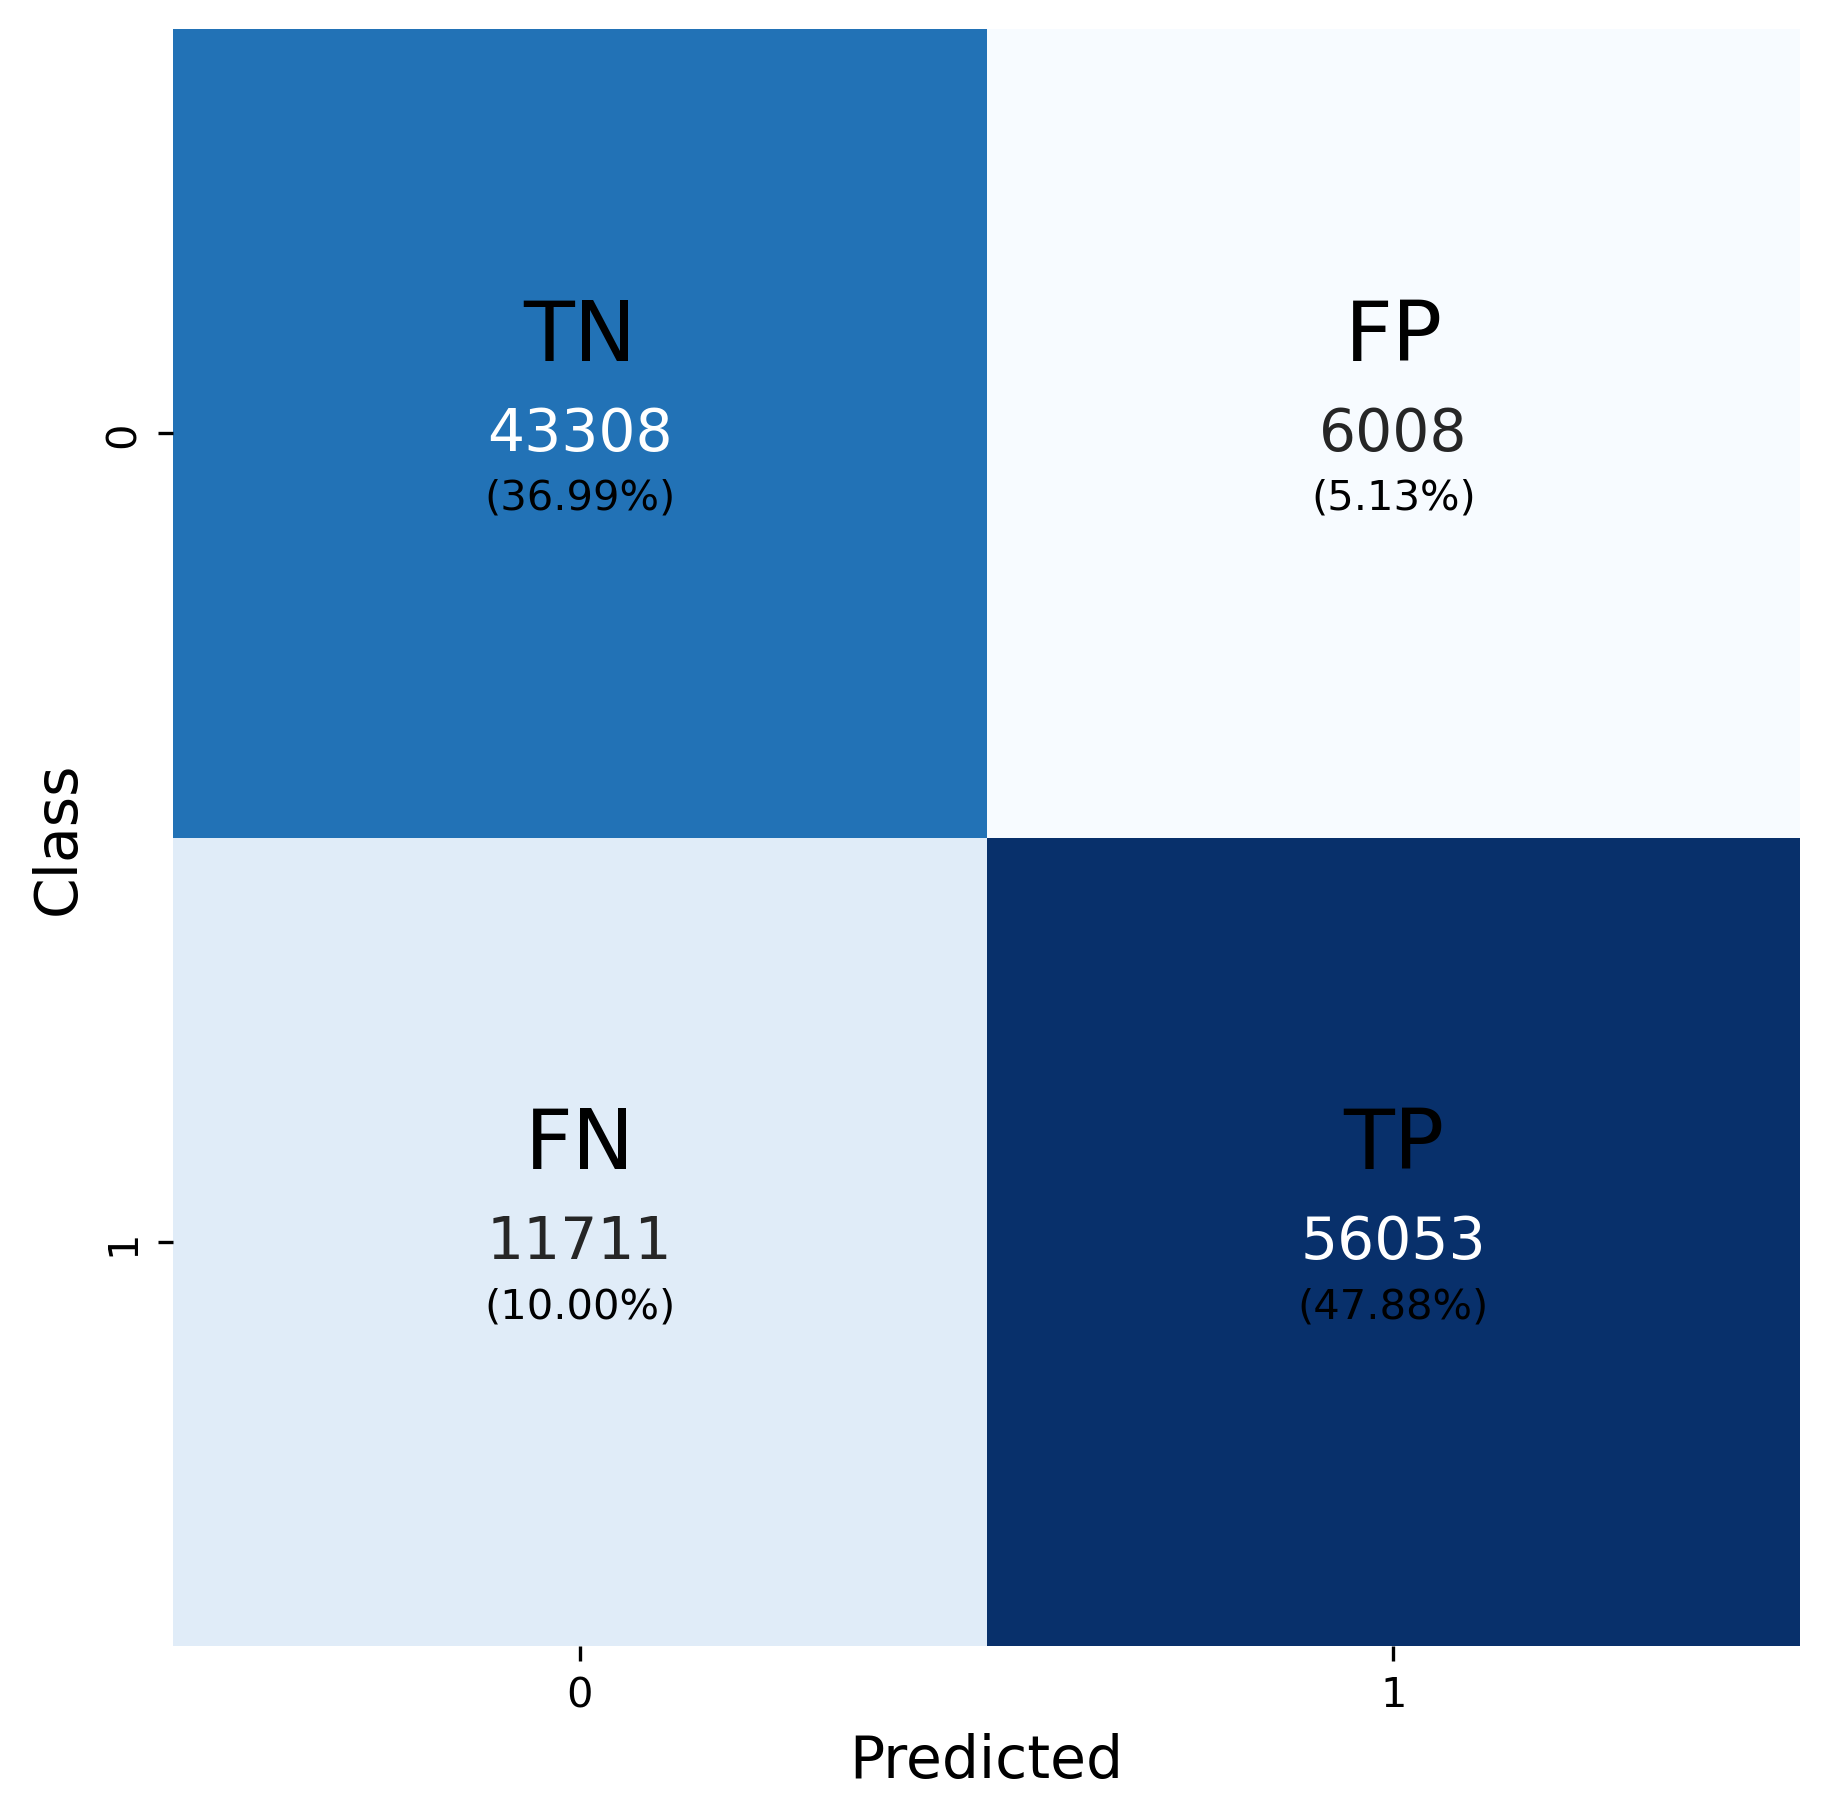
\includegraphics[width=0.45\columnwidth,angle=0]{confusion_matrix_knn.png}
    \caption[]{Matriz de confusão do modelo KNN. A diagonal principal representa os valores corretamente classificados, enquanto os valores fora da diagonal principal representam os erros de classificação das classes 0 e 1.}
    \label{confusion_matrix_knn}
\end{figure}

\vspace{\baselineskip}

Muitos dos objetos tiveram classificação correta, como podemos ver na diagonal principal da matriz de confusão. Porém, cabe ressaltar que nem todos os objetos do conjunto de teste eram estrelas ou galáxias, e sim com majoritariamente mais de cada um deles nas classes de compactos e extensos, respectivamente. Assim é esperado que algumas classificações sejam feitas de forma errada, e é nessa proposta que o modelo foi treinado, encontrar aqueles com maior probabilidade de serem extensos mas fazem parte do conjunto dos compactos.

\vspace{\baselineskip}

Usamos ainda as métricas de acurácia, precisão, recall e F1-score para avaliar o desempenho do modelo.

A acurácia é definida como a fração das previsões corretas em relação ao total. 

\begin{equation}
    \text{Acurácia} = \frac{TP + TN}{TP + TN + FP + FN}
\end{equation}

A precisão é a fração de verdadeiros positivos em relação ao total de positivos. 

\begin{equation}
    \text{Precisão} = \frac{TP}{TP + FP}
\end{equation}

O recall (ou completeza) é a fração de verdadeiros positivos em relação ao total de positivos previstos.

\begin{equation}
    \text{Recall} = \frac{TP}{TP + FN}
\end{equation}

O F1-score é a média harmônica entre precisão e recall.

\begin{equation}
    \text{F1-score} = 2 \times \frac{\text{Precisão} \times \text{Recall}}{\text{Precisão} + \text{Recall}}
\end{equation}

Usamos ainda a curva a curva AUC-ROC, bem utilizada para modelos de classificação binária. A ROC (Receiver Operating Characteristic) exibe a relação entre a sensibilidade (taxa de verdadeiros positivos) e a taxa de falsos positivos para diferentes valores. A AUC (Área Sob a Curva) resume como a performance foi em um único valor: quanto mais próxima ela está de 1, melhor o modelo diferencia entre as classes. Uma AUC de 0.5 indica classificação aleatória, enquanto 1.0 representa um modelo perfeito.

\vspace{\baselineskip}

Essas são as métricas mais populares adotadas em tarefas de classificação binária. Porém, essas medidas estatísticas podem mostrar resultados excessivamente otimistas, especialmente em conjuntos de dados desbalanceados. Uma métrica adicional que usaremos é o coeficiente de correlação de Matthews (MCC), definido por:

\begin{equation}
    \text{MCC} = \frac{TP \times TN - FP \times FN}{\sqrt{(TP + FP)(TP + FN)(TN + FP)(TN + FN)}}
\end{equation}

Ele é uma taxa estatística mais confiável que produz uma pontuação alta apenas se a previsão obtiver bons resultados em todas as quatro categorias da matriz de confusão, proporcionalmente tanto ao tamanho dos elementos positivos quanto ao tamanho dos elementos negativos no conjunto de dados. Os valores do MCC variam de -1 a 1, em que 1 indica uma previsão perfeita, 0 indica uma previsão aleatória e -1 indica uma previsão totalmente incorreta.


A tabela \ref{metricas_modelo} mostra as métricas obtidas para o modelo KNN treinado.

\begin{table}[!ht]
    \centering
    \caption{Classificação binária - Métricas modelo KNN}
    \begin{tabular}{lccc}
        \toprule
        Classe & Precisão & Recall & F1-Score \\
        \midrule
        0 & 0.80 & 0.88 & 0.83 \\
        1 & 0.90 & 0.83 & 0.86 \\
        \midrule
        \multicolumn{3}{l}{AUC-ROC} & 0.91 \\
        \multicolumn{3}{l}{Coeficiente de Correlação de Matthews (MCC)} & 0.70 \\
        \bottomrule
    \end{tabular}
    \label{metricas_modelo}
\end{table}

Os resultados obtidos têm valores de precisão, recall e F1-score acima de 0.8 para ambas as classes. A AUC-ROC de 0.93 indica que o modelo é capaz de distinguir entre as duas classes com boa precisão dada as limitações dos conjuntos de treinamento. O coeficiente de correlação de Matthews (MCC) de 0.70 é um indicativo de que o modelo é capaz de prever corretamente a maioria dos objetos.

\vspace{\baselineskip}

A principal dificuldade com o classificador está nas regiões onde as classes se sobrepõem no gráfico da Figura \ref{distribution_of_stars_and_galaxies}. No entanto, esperamos que o classificador tenha um desempenho melhor nas regiões onde há uma maior concentração de uma única classe no bin de \textit{FWHM}. As classificações e o treinamento do modelo devem refletir essa expectativa.
Foi realizada as previsões de probabilidade de ser da classe 1 (objetos extensos) para toda a amostra que estaremos analisando a busca (amostra de treino e amostra de teste). 
A Figura \ref{probabilidade_extensos_fwhm} mostra a distribuição de \textit{FWHM} na banda \textit{r} dos objetos com classificação estrela-galáxia do GAIA DR3 com probabilidade maior que 90\%. Sobreposto na imagem temos matrizes de confusão do classificador para diferentes intervalos de \textit{FWHM}.

\begin{figure}[!ht]
    \centering
    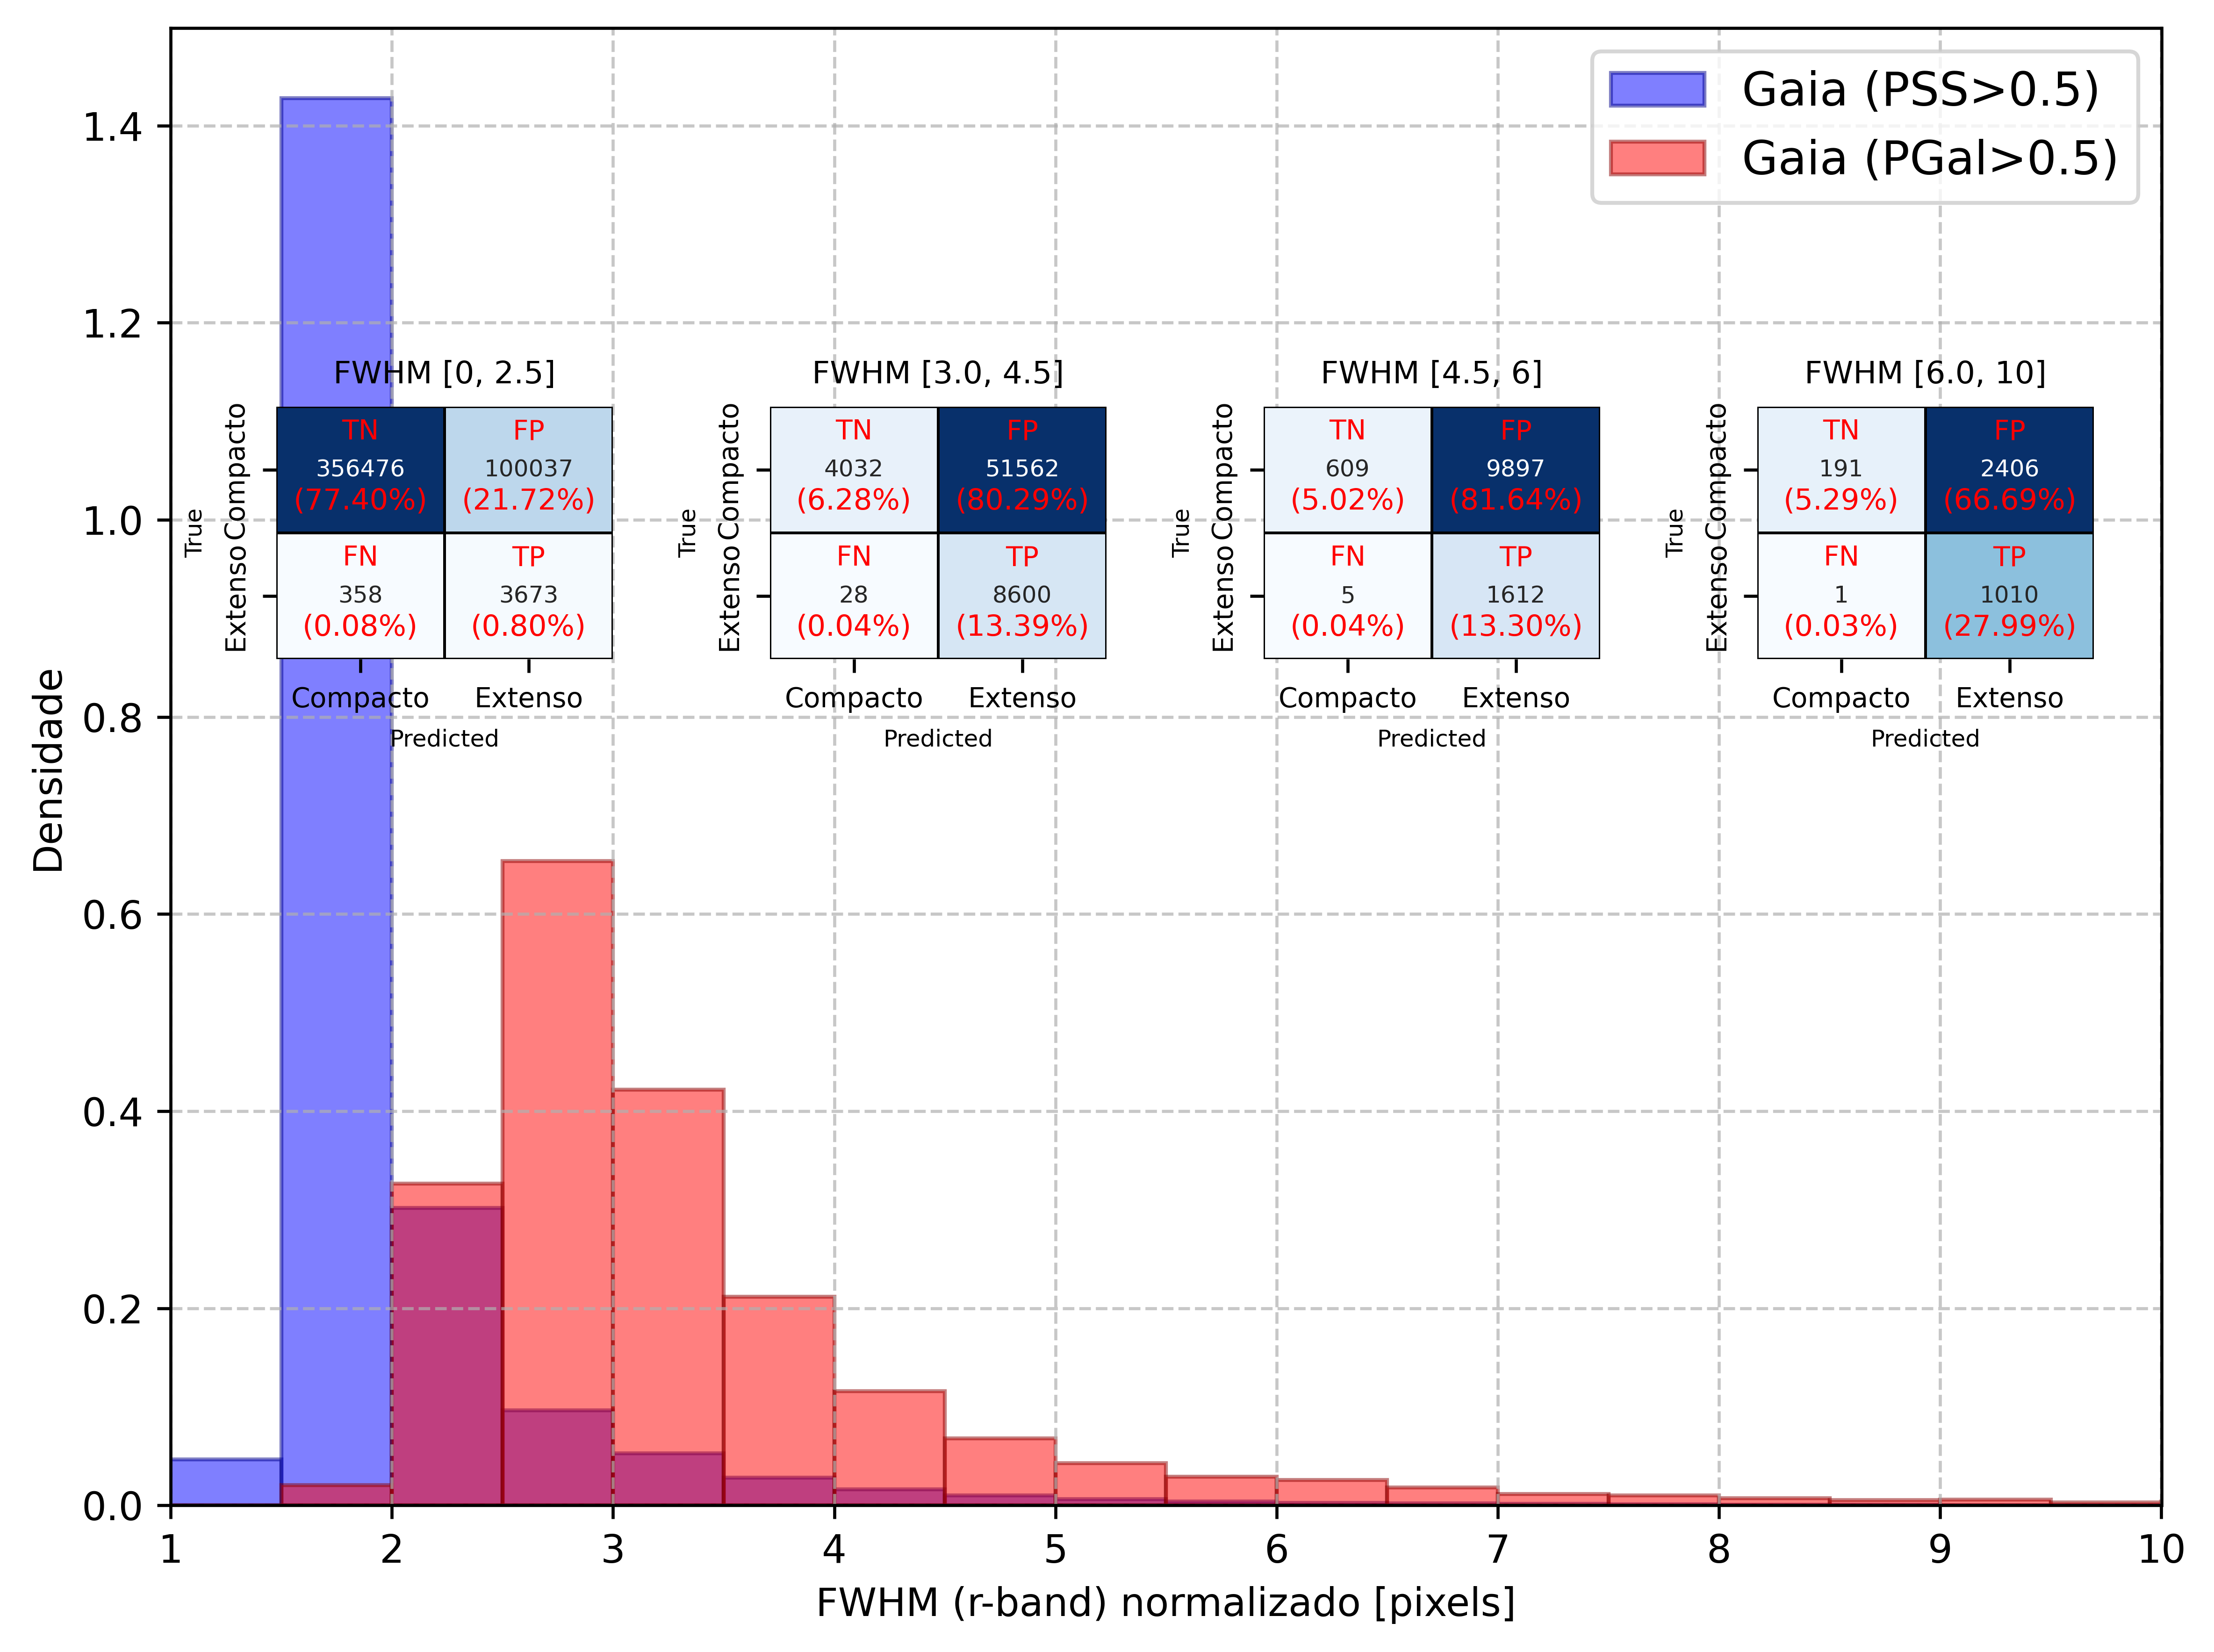
\includegraphics[width=0.95\columnwidth,angle=0]{distribution_of_stars_and_galaxies_with_cm.png}
    \caption[]{Distribuição de \textit{FWHM (r-band)} para objetos da amostra com classificação estrela-galáxia do GAIA DR3 com probabilidade maior que 90\%. As matrizes de confusão do classificador KNN para diferentes intervalos de \textit{FWHM} são sobrepostas.}
    \label{probabilidade_extensos_fwhm}
\end{figure}

\vspace{\baselineskip}

O comportamento do classificador nas matrizes de confusão mostra que, para as regiões de \textit{FWHM} menores (entre [0, 3]), onde têm uma maior concentração de estrelas, se observa uma alta taxa de classificação para objetos do tipo compacto. Já para objetos com \textit{FWHM} maiores, o classificador mostra uma tendência de classificá-los como extensos, o que é esperado, já que esses objetos são menos prováveis de serem estrelas. Para objetos com \textit{FWHM} nas faixas de sobreposição, o desempenho do classificador é misto, refletindo a dificuldade em separar essas classes na região. Porém, é possível observar uma transição gradual entre as classes, consistente com os picos das distribuições de \textit{FWHM}.

\vspace{\baselineskip}

Ilustrando ainda o resultado da classificação, apresentamos na Figura \ref{predic_colored} o mesmo gráfico da Figura \ref{amostra_treino} para os objetos da amostra de teste, coloridos de acordo com a probabilidade de serem objetos extensos pelo modelo. A cor azul indica uma probabilidade baixa, enquanto a cor vermelha indica uma probabilidade alta.


\begin{figure}[!ht]
    \centering
    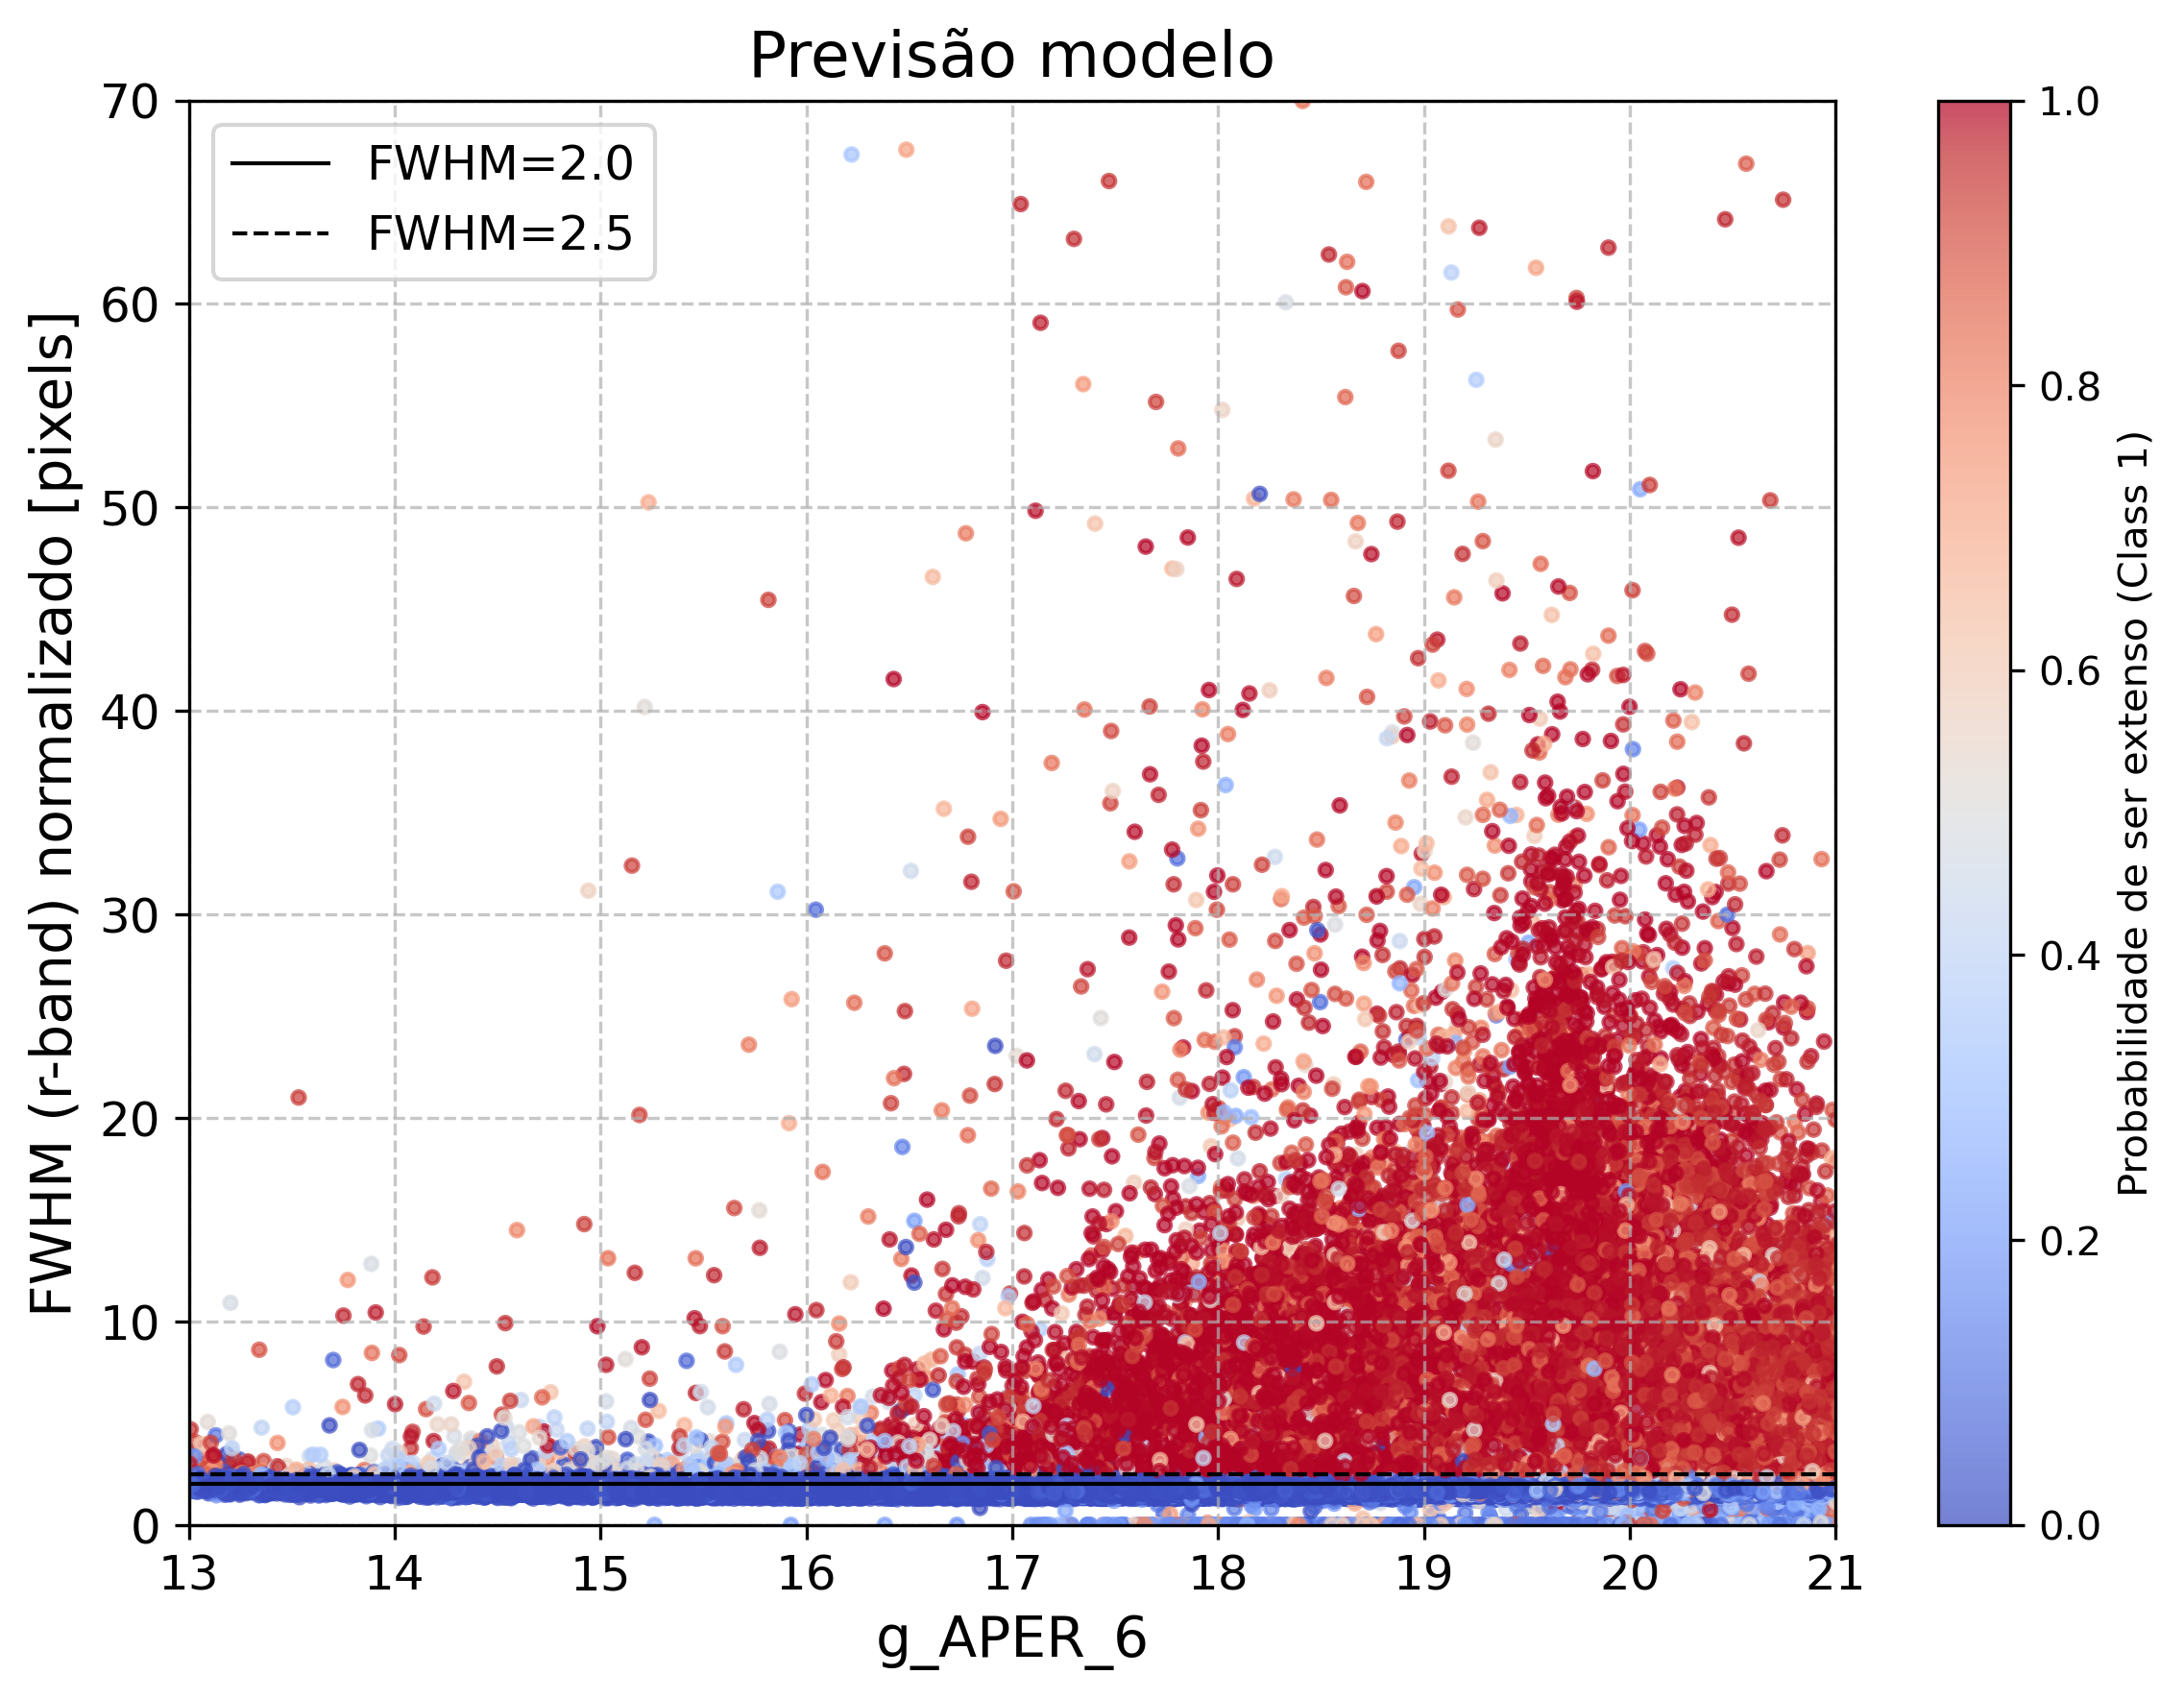
\includegraphics[width=0.95\columnwidth,angle=0]{predic_colored.png}
    \caption[]{Distribuição da Largura Total na Metade Máxima (\textit{FWHM} r-band) em função da magnitude \textit{g\_PETRO} para objetos da amostra de teste, coloridos de acordo com a probabilidade de serem objetos extensos (Class 1) pelo modelo. Divisão das classes: compactos (\textit{FWHM}$\leq$3 pixels) e extensos (\textit{FWHM}$\geq$3.5 pixels).}
    \label{predic_colored}
\end{figure}

\vspace{\baselineskip}

A probabilidade dos objetos serem da classe 1 (objetos extensos) para as UCDs presentes na amostra é apresentada na Tabela \ref{ucds_predict}.

\begin{table}[H]
    \centering
    \caption{Classificação do modelo se ser da classe 1 (objetos extensos) das UCDs na amostra de análise}
    \begin{tabular}{lc}
        \toprule
        Nome & Predição  \\
        \midrule
        UCD3 & 0.07 \\
        F-1a & 0.06 \\
        F-24 & 1.00 \\
        UCD1 & 1.00 \\
        UCD5 & 1.00 \\
        F-5 & 1.00 \\
        F-12 & 1.00 \\
        F-9 & 1.00 \\
        \midrule
    \end{tabular}
    \label{ucds_predict}
\end{table}

Das 8 UCDs presentes, 6 foram classificadas com uma predição excelente, de 100\%, e 2 com classificação muito pouco provável. Dessa forma recuperamos a maioria dos objetos de interesse, mostrando a eficácia para buscar novos na amostra.

\section{Seleção das candidatas}\label{cap:selecao_candidatas}
Para a seleção das candidatas, queremos primeiramente criar uma subamostra dos dados de Fornax, contendo os objetos compactos de nosso interesse. A partir dessa amostra, iremos selecionar pelas probabilidades de serem extensos (classe 1).

\vspace{\baselineskip}

Inicialmente, removemos os objetos que possuem classificação pelo GAIA acima de 50\% de serem estrelas, diminuindo um pouco a contaminação. A partir de \cite{Su_2021}, removemos também os objetos confirmados espectroscopicamente como sendo do background. Usando o catálogo de redshifts espectroscópicos de \cite{Lima_2024}, removemos os objetos que possuem redshifts maiores que 0.0055, considerando que esses objetos estão mais distantes de Fornax e, portanto, não pertencem ao aglomerado.

\vspace{\baselineskip}

Para a seleção dos objetos compactos, cortamos na magnitude \textit{g\_PETRO}$\geq$13, evitando objetos mais brilhantes e saturados. Cortamos também \textit{g\_PETRO}$\leq$21, para evitar a contaminação de aglomerados globulares. Cortamos nas 12 magnitudes da abertura PETRO em magnitudes maiores do que 30, evitando objetos com baixa qualidade de medição, com erros fotométricos altos. Cortamos também em cada uma das mesmas bandas valores de \textit{flag0}$\leq$2, que são objetos com problemas de qualidade de medição.

\vspace{\baselineskip}

Pela Figura \ref{distribuicao_fwhm_image_r_r_petro_ucds_fornax}, das UCDs conhecidas em Fornax, cortamos pela magnitude \textit{r\_PETRO}$\geq$17, correspondendo a 0.5 magnitudes de diferença da UCD mais brilhante no intervalo. 
Das 8 UCDs conhecidas em Fornax, temos o maior \textit{FWHM (r-band)} para a \textit{UCD3} com 4.49 pixels, 6 delas sendo menores que 4 pixels. Assim, para a seleção dos objetos compactos, cortamos em \text{FWHM (r-band)}$\leq$4.4 pixels.

\vspace{\baselineskip}

Esperamos que os objetos compactos, como as UCDs, tenham uma distribuição mais pontual e, assim, menos elíptica do que comparado a galáxias disco ou elípticas. Das 7 UCDs conhecidas que permaneceram na nossa amostra após as seleções, a partir do parâmetro \text{ELLIPTICITY}, todas têm valores abaixo de 0.11. Adotamos uma seleção com \text{ELLIPTICITY} $\leq$ 0.2, removendo objetos que possuíam algum formato de disco.

\vspace{\baselineskip}

Usando os parâmetros \text{FLUX\_RADIUS\_90}, \text{FLUX\_RADIUS\_70}, \text{FLUX\_RADIUS\_50} e \text{FLUX\_RADIUS\_20}, que correspondem à medida em pixels do raio que contém 90\%, 70\%, 50\% e 20\% do fluxo total da fonte, respectivamente, esperamos que as UCDs tenham uma distribuição mais pontual. Dessa forma, em diferentes distâncias radiais, por exemplo, entre 90\% e 70\%, devemos esperar que existam certas diferenças nas distribuições de luz das UCDs, estrelas e algumas galáxias mais extensas. Com essa ideia, criamos alguns gráficos com as melhores combinações de parâmetros que ajudam a remover a contaminação na amostra. Mostramos nas Figuras \ref{flux_radius_1}, \ref{flux_radius_2} e \ref{flux_radius_3} os três gráficos com a combinação de parâmetros. 

Em cada uma das 3 figuras, foram delimitadas visualmente duas retas, dividindo as fronteiras com para galáxias e estrelas. Assim temos 6 outros cortes realizados para remover a contaminação de candidatas indesejadas.

\begin{figure}[!ht]
    \begin{center}
    % \setcaptionmargin{1cm}
    \includegraphics[width=0.75\columnwidth,angle=0]{f_90_20_R_PETRO_c.png}
    \caption{Gráfico de \text{FLUX\_RADIUS\_90} - \text{FLUX\_RADIUS\_70} (f\_90\_70) em função de \text{r\_PETRO} para objetos da amostra com classificação estrela-galáxia do GAIA DR3 com probabilidade maior que 90\%. Pontos em azul as estrelas, em vermelho as galáxias e em petro as UCDs. Retas em verde e roxo representar os cortes para remover as contaminação de estrelas.}
    \label{flux_radius_1}
    \end{center}
\end{figure}

\vspace{\baselineskip}

\begin{figure}[!ht]
    \begin{center}
    % \setcaptionmargin{1cm}
    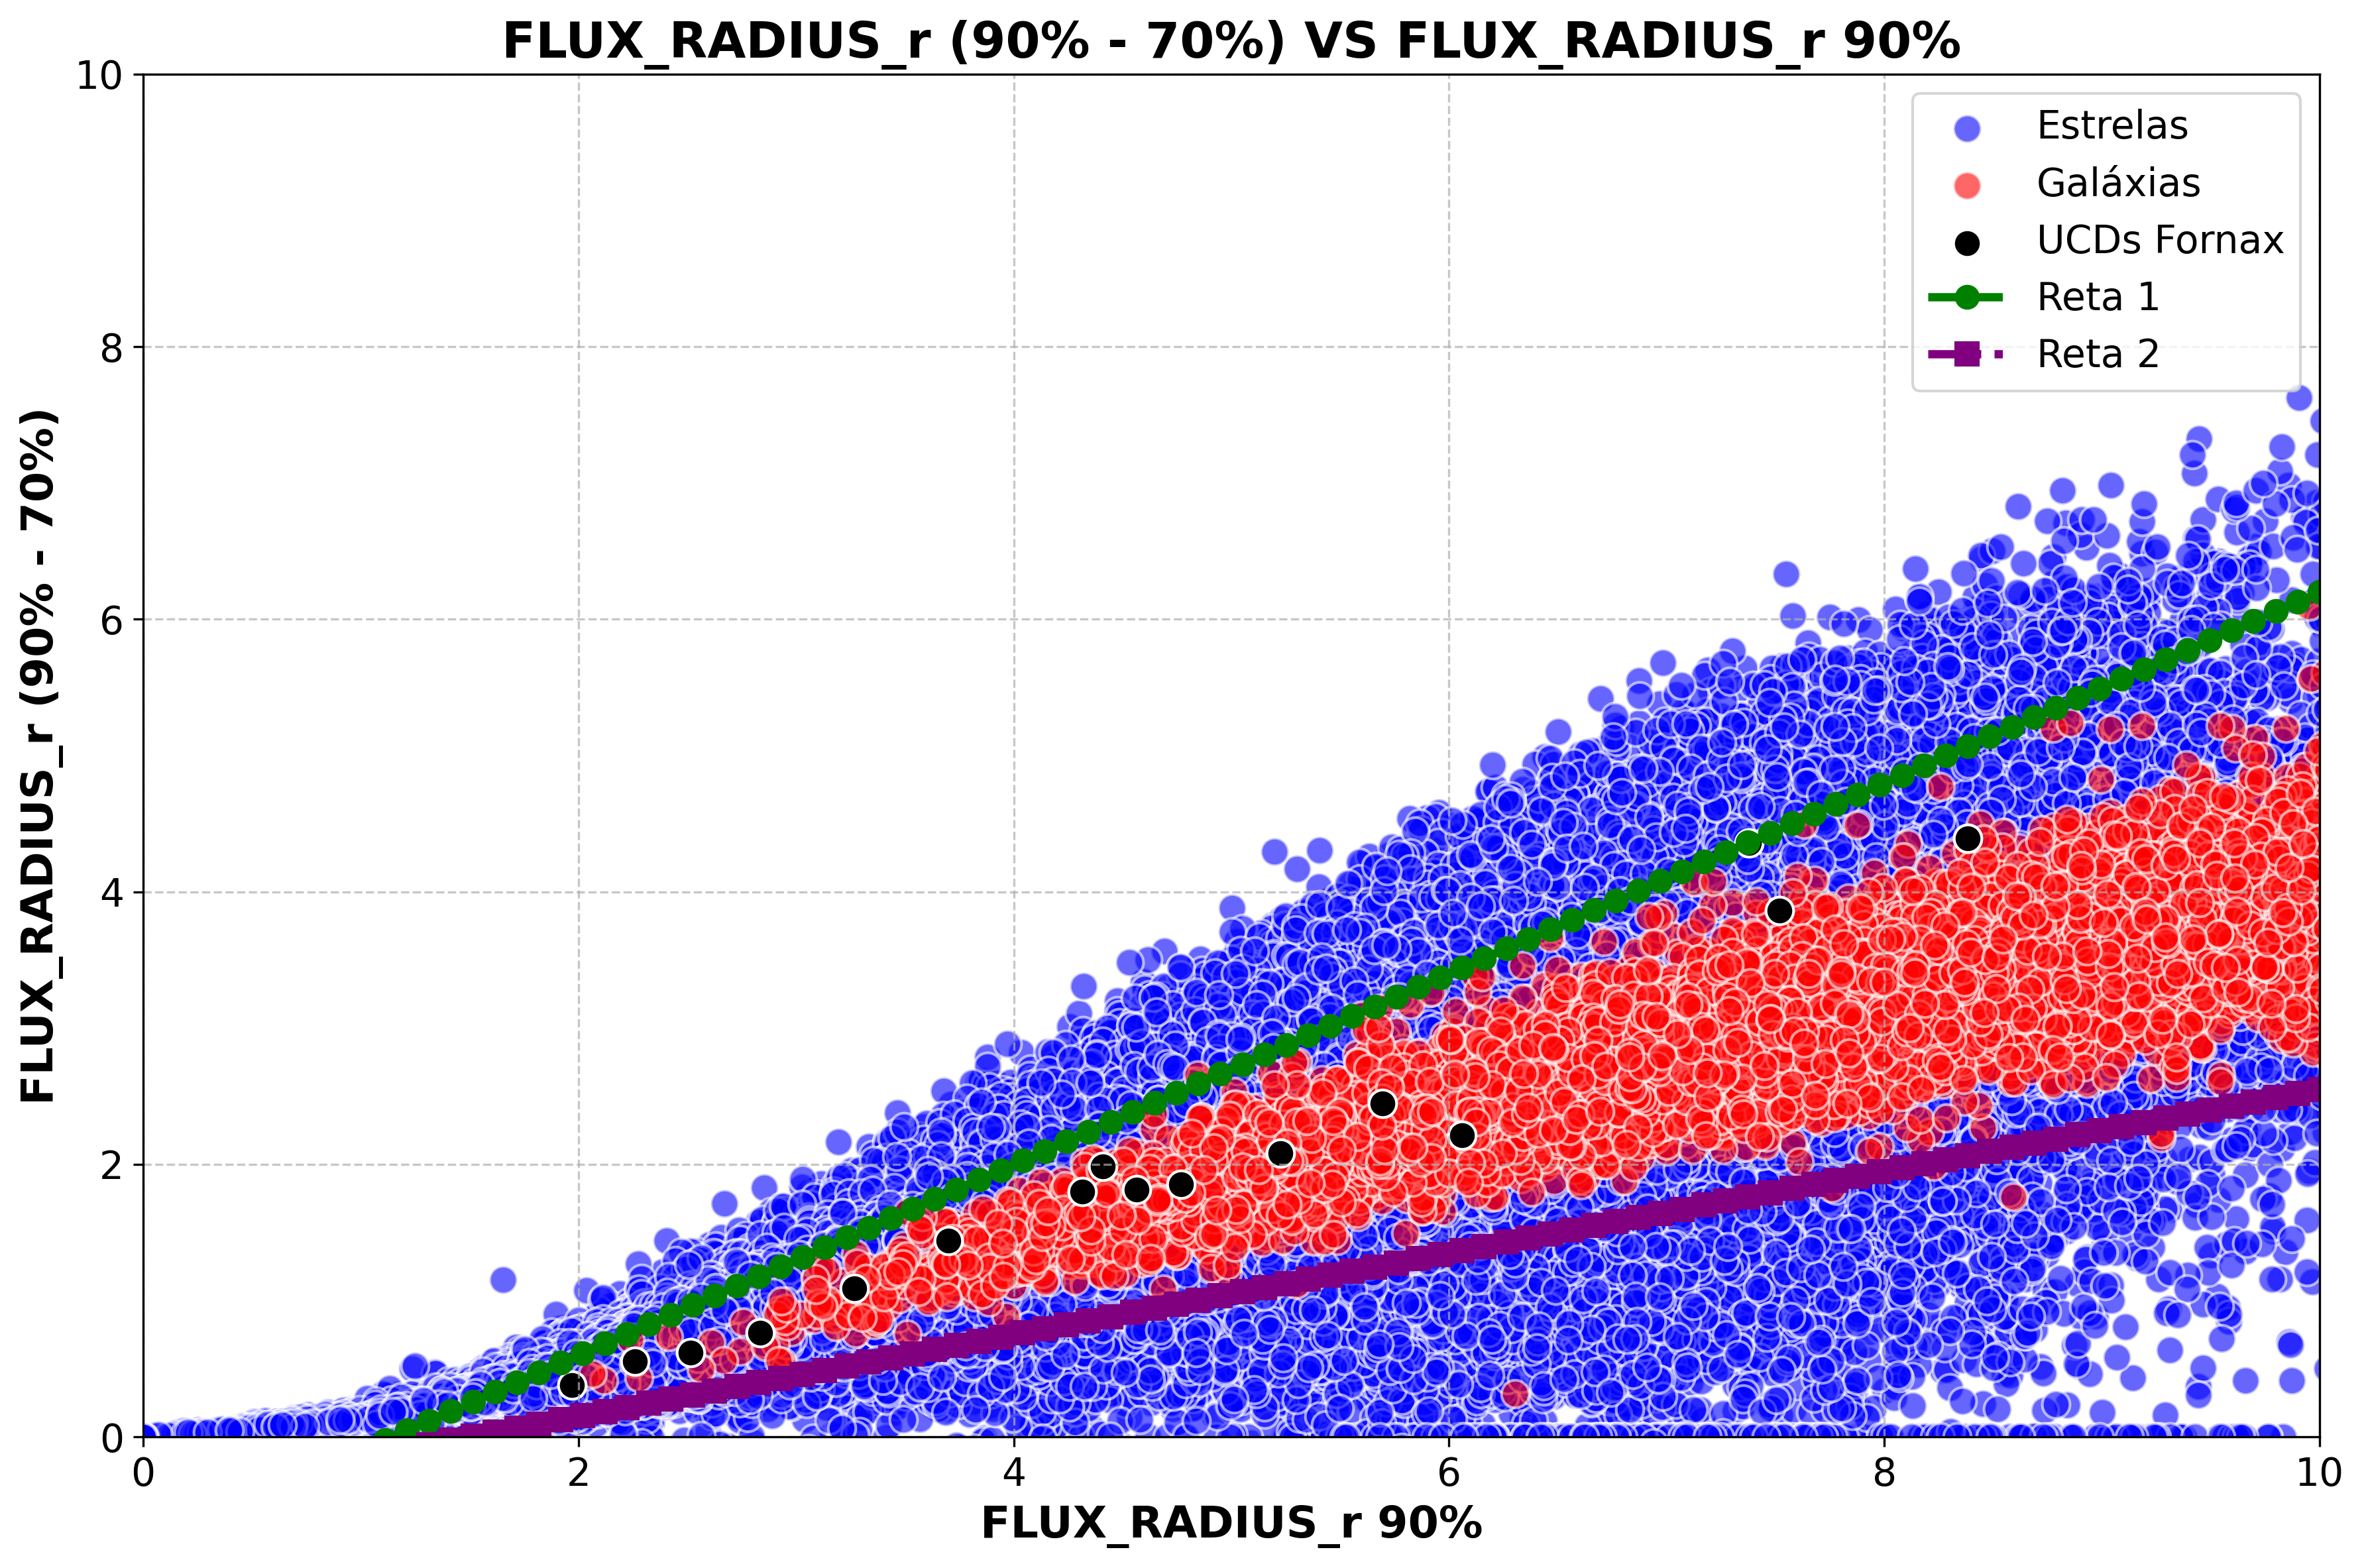
\includegraphics[width=0.75\columnwidth,angle=0]{f_90_70_FLUX_RADIUS_90_R.png}
    \caption[]{Gráfico de \text{FLUX\_RADIUS\_70} - \text{FLUX\_RADIUS\_20} (f\_70\_20) em função de \text{FLUX\_RADIUS\_90} - \text{FLUX\_RADIUS\_70} (f\_90\_70) para objetos da amostra com classificação estrela-galáxia do GAIA DR3 com probabilidade maior que 90\%. Pontos em azul as estrelas, em vermelho as galáxias e em petro as UCDs. Retas em verde e roxo representar os cortes para remover as contaminação de estrelas.}
    \label{flux_radius_2}
    \end{center}
\end{figure}

\vspace{\baselineskip}

\begin{figure}[!ht]
    \begin{center}
    % \setcaptionmargin{1cm}
    \includegraphics[width=0.75\columnwidth,angle=0]{f_70_20_f_90_70.png}
    \caption[]{Gráfico de \text{FLUX\_RADIUS\_90} - \text{FLUX\_RADIUS\_70} (f\_90\_70) em função de \text{FLUX\_RADIUS\_90} para objetos da amostra com classificação estrela-galáxia do GAIA DR3 com probabilidade maior que 90\%. Pontos em azul as estrelas, em vermelho as galáxias e em petro as UCDs. Retas em verde e roxo representar os cortes para remover as contaminação de estrelas.}
    \label{flux_radius_3}
    \end{center}
\end{figure}

\vspace{\baselineskip}

Depois desses cortes para seleção de objetos compactos, dados as classificações do modelo, filtramos aqueles com probabilidade maior que 90\% de serem extensos. A partir dessa amostra, selecionamos as candidatas a UCDs, que são objetos compactos com alta probabilidade de serem extensos.

\vspace{\baselineskip}

Ao final de todo o processo de seleção de candidatas com maiores similaridades com as UCDs, encontramos um total de 7081 objetos de uma amostra inicial de $\sim$ 2.9 milhões de objetos em Fornax. 

\section{Redshifts fotométricos}
Com os objetos filtrados de candidatas, temos uma amostra menor (7081 objetos), porém ainda relativamente grande para uma análise mias detalhada. Para reduzir ainda mais a amostra, calculamos redshifts fotométricos (\textit{$z_{phot}$}) desses objetos, selecionando aqueles nos intervalos mais compatíveis com Fornax.

\vspace{\baselineskip}

É possível encontrar redshifts fotométricos para parte dos objetos da nossa amostra em outros trabalhos da literatura, assim como em catálogos da própria colaboração S-PLUS. Porém, para a buscar nesse projeto, utilizamos dados com a redução da fotometria do S-PLUS diferentes dos utilizados para os \textit{$z_{phot}$} disponíveis. Assim, recalculamos os redshifts fotométricos para a nossa amostra.

\vspace{\baselineskip}

Abordagens para calcular \textit{$z_{phot}$} comuns envolvem o ajuste a partir de modelos (\textit{template fitting}) ou por técnicas de aprendizado de máquina. A predição feita por \textit{template fitting} tem suas vantagens ao conseguir extrapolar resultados desejados. Já o aprendizado de máquina, por outro lado, é mais confiável dentro de um intervalo dado o seu conjunto de treinamento, além de ter a vantagem de ser mais rápido e preciso, desde que o conjunto de treinamento seja representativo.

\vspace{\baselineskip}

Aqui optamos por utilizar o método de aprendizado de máquina para calcular \textit{$z_{phot}$}. Para isso, empregamos modelos de regressão utilizando o algoritmo K-Nearest Neighbors (KNN), implementado em Python. No caso da regressão, o KNN prevê valores contínuos ao calcular a média dos valores-alvo dos \textit{K} vizinhos mais próximos no espaço de características.

\vspace{\baselineskip}

Para a seleção da amostra de treino, utilizamos o mesmo catálogo de Fornax usados anteriormente, com os dados de fotometria do S-PLUS provenientes de \cite{haack2024splusfornaxprojectsfp} (\textit{Run 1}). Isso é, temos os mesmo dados como descritos na sessão \ref{sec:Fornax_data}, com as 12 magnitudes com correção de extinção (como descritas na sessão \ref{sec:Coeficientes_ext}).

\vspace{\baselineskip}

Dessa amostra, selecionamos os objetos com redshifts espectroscópicos disponíveis, provenientes do catálogo \cite{Lima_2024}. Cortamos os objetos em um intervalo de redshifts de 0.002 a 0.4, dessa maneira evitamos boa partes das estrelas (com redshifts menores) e galáxias mais distantes de Fornax. Cortamos também em um intervalo de magnitude de \textit{r\_AUTO}$\geq$15 e \textit{r\_AUTO}$\leq$20, evitando objetos muito brilhantes e saturados, e objetos com baixa qualidade de medição, respectivamente. 

\vspace{\baselineskip}

Removemos ainda os objetos com medições faltantes em alguma das 12 magnitudes das aberturas \textit{PETRO}, e ao final, temos uma amostra com 8789 objetos.

\vspace{\baselineskip}

Para o treinamentos, os melhores resultados a principio se deram com a utilização das combinações das 66 cores das 12 magnitudes de abertura \textit{PETRO}. Assim treinamos o modelo provendo o redshift espectroscópico (\textit{$z_{spec}$}.) como variável alvo e as 66 cores como variáveis preditoras.

\vspace{\baselineskip}

A seleção dos melhores hiperparâmetros foi realizada com validação cruzada de 5 folds, otimizando os parâmetros \textit{n\_neighbors}, \textit{metric}, \textit{weights}, \textit{algorithm} e \textit{leaf\_size}.

\vspace{\baselineskip}

O modelo final selecionado foi treinado com 18 vizinhos, utilizando a distância de euclidiana como métrica, pesos proporcionais à distância, \textit{algorithm}='auto' e \textit{leaf\_size}=10. Além disso, o conjunto de dados foi normalizado com base na amostra de treino, ajustando sua distribuição para valores entre 0 e 1, de forma a garantir a correta aplicação das métricas de distância. Além disso, dividimos a amostra de treino e teste em 80\% e 20\%, respectivamente.

\vspace{\baselineskip}

A Figura \ref{zphot_zspec} mostra a comparação entre os redshifts espectroscópicos ($\textit{$z_{spec}$}$) e fotométricos (\textit{$z_{phot}$}) para a amostra de treino. A linha tracejada representa a relação 1:1 entre os redshifts, enquanto a linha contínua representa a relação ajustada pelo modelo de regressão.

\begin{figure}[!ht]
    \centering
    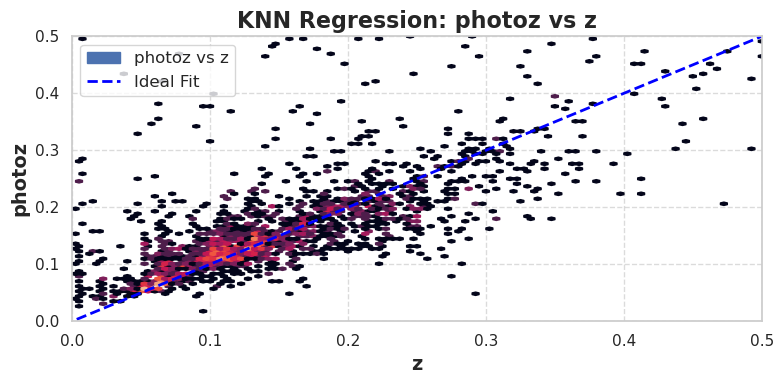
\includegraphics[width=1.\columnwidth,angle=0]{zphot_zspec.png}
    \caption[]{Resultados da regressão com o algoritmo K-Nearest Neighbors (KNN) para estimar os redshifts fotométricos (\textit{$z_{phot}$}) em relação aos redshifts espectroscópicos (\textit{$z_{spec}$}). Na parte superior, o gráfico de dispersão compara \textit{$z_{phot}$} vc \textit{$z_{spec}$}. A linha azul tracejada representa o ajuste ideal ( \textit{$z_{phot}$} = \textit{$z_{spec}$}). A densidade de pontos é representada por um gradiente de cores, com áreas mais densas indicadas em tons mais claros. Na parte inferior, o gráfico de resíduos exibe a diferença entre \textit{$z_{phot}$} e \textit{$z_{spec}$}. A linha preta tracejada representa a linha zero.}
    \label{zphot_zspec}
\end{figure}

\vspace{\baselineskip}

Percebemos pela Figura \ref{zphot_zspec} que o modelo de regressão foi capaz de estimar os redshifts fotométricos com alguma certa precisão. Porém ainda temos algumas estimativas com erros maiores, principalmente para redshifts mais altos. Porém, vale ressaltar que não queremos com esse modelo estimar redshifts precisos para todos os objetos, mas sim selecionar aqueles com redshifts compatíveis com Fornax. Assim, mesmo com erros, se pudermos usar o modelo para remover objetos com redshifts com as maiores probabilidades de serem do fundo, já teremos um grande ganho.

\vspace{\baselineskip}

Aplicando o modelo para as UCDs conhecidas em Fornax que adotamos para a análise, temos os resultados apresentados na Tabela \ref{ucds_zphot}.

\begin{table}[!ht]
    \centering
    \caption{Aplicação do modelo de regressão para estimativas de redshifts fotométricos paras UCDs conhecidas na amostra de análise de Fornax}
    \begin{tabular}{lc}
        \toprule
        Nome & \textit{$z_{phot}$}   \\
        \midrule
        UCD3 & 0.005 \\
        F-1a & 0.132 \\
        F-24 & 0.111 \\
        UCD1 & 0.005 \\
        UCD5 & 0.136 \\
        F-5 & 0.005 \\
        F-12 & 0.005 \\
        F-9 & 0.146 \\
        \midrule
    \end{tabular}
    \label{ucds_zphot}
\end{table}

Dado que essas UCDs são conhecidas em Fornax, esperamos que os redshifts fotométricos sejam compatíveis com o aglomerado. Sabendo que o redshift de Fornax é de $\sim 0.005$\footnote{https://simbad.u-strasbg.fr/simbad/sim-id?Ident=Fornax+Cluster}, é interessante notar que na Tabela \ref{ucds_zphot}, dos 8 objetos, 4 tiveram predições compatíveis com o aglomerado, enquanto 4 tiveram redshifts mais altos. 

\vspace{\baselineskip}

Podemos interpretar que, de certa maneira, algumas dessa UCDs, no espaço de parâmetros das cores treinadas, têm características mais próximas de objetos do fundo. Assim, seria necessária uma análise mais detalhada das diferenças desses dois grupos de UCDs, quando comparadas com os redshifts fotométricos previsto. Mas de qualquer forma, interpretamos que, adotando um corte conservador para os redshifts fotométricos, podemos remover objetos com maiores chances de serem do fundo, e selecionar possíveis candidatas a UCDs, sabendo que podemos estar perdendo ainda este possível outro grupo de UCDs com estimativas de redshifts mais altas.

\vspace{\baselineskip}

Aplicando o modelo então na amostra de candidatas, calculando os redshifts fotométricos para os 7081 objetos. A partir desses redshifts, adotados um corte para remover os objetos com maiores chances de serem do fundo do aglomerado. Dado o valor do redshift de Fornax de $\sim 0.005$, adotamos um corte com uma margem otimista para o erro, cortando em \textit{$z_{phot}$}$\leq$0.055.

\section{Análise das candidatas}

\section{Candidatas para espectroscopia}
Nesta sessão, iremos discutir sobre os objetos selecionados para a espectroscopia ao longo do projeto. Dando sequência à um projeto anterior de iniciação cientifica, foram selecionadas 18 candidatas a UCDs. Foi submetido na época do projeto um pedido de tempo ao telescópio Gemini Sul, para observação espectroscópica com o GMOS. Até o momento, foram observadas 14 delas. Como parte do inicio deste projeto, foi feito a aquisição desses objetos para análise dos espectros.

\vspace{\baselineskip}

Na tabela \ref{candidatas_espectroscopia_1} temos a lista dessas candidatas observadas, com suas respectivas coordenadas. Utilizando o Legacy Survey Sky Browser\footnote{Legacy Survey Sky Browser}, apresentamos na Figura \ref{candidatas_espectroscopia_1_img} as imagens desse objetos.

\begin{table}[!ht]
    \centering
    \caption{Conjunto de candidatas a UCDs observadas com o GMOS no telescópio Gemini Sul selecionadas de um projeto anterior. Coluna $OBJ_{name}$ é o nome interno da candidata utilizado no pedido de tempo do Gemini.}
    \begin{tabular}{lcc}
        \toprule
        $OBJ_{name}$ & RA     & DEC     \\
        \midrule
        UCG01     & 47,708 & -34,157 \\
        UCG02     & 47,960 & -33,174 \\
        UCG03     & 49,910 & -31,523 \\
        UCG04     & 53,753 & -37,155 \\
        UCG05     & 53,820 & -35,837 \\
        UCG06     & 54,115 & -36,845 \\
        UCG07     & 54,214 & -36,814 \\
        UCG08     & 54,912 & -35,439 \\
        UCG09     & 55,010 & -35,535 \\
        UCG10     & 55,056 & -37,895 \\
        UCG11     & 55,211 & -38,048 \\
        UCG12     & 55,315 & -37,020 \\
        UCG13     & 55,333 & -36,653 \\
        UCG14     & 55,673 & -36,541 \\
        UCG15     & 57,272 & -35,515 \\
        UCG16     & 57,468 & -34,663 \\
        UCG17     & 58,035 & -37,111 \\
        UCG18     & 58,083 & -36,298 \\
        \bottomrule
    \end{tabular}
    \label{candidatas_espectroscopia_1}
\end{table}


\begin{figure}[!ht]
    \centering
    \captionsetup{justification=centering}
    \begin{subfigure}[b]{0.22\textwidth}
        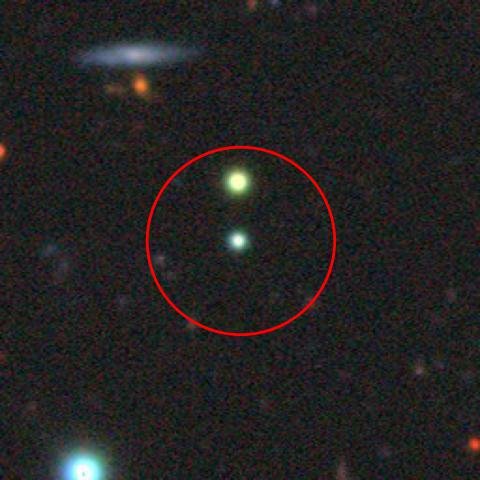
\includegraphics[width=\textwidth]{proposatal_candidatas_1/UCG01.png}
        \caption{UCG01}
    \end{subfigure}
    \begin{subfigure}[b]{0.22\textwidth}
        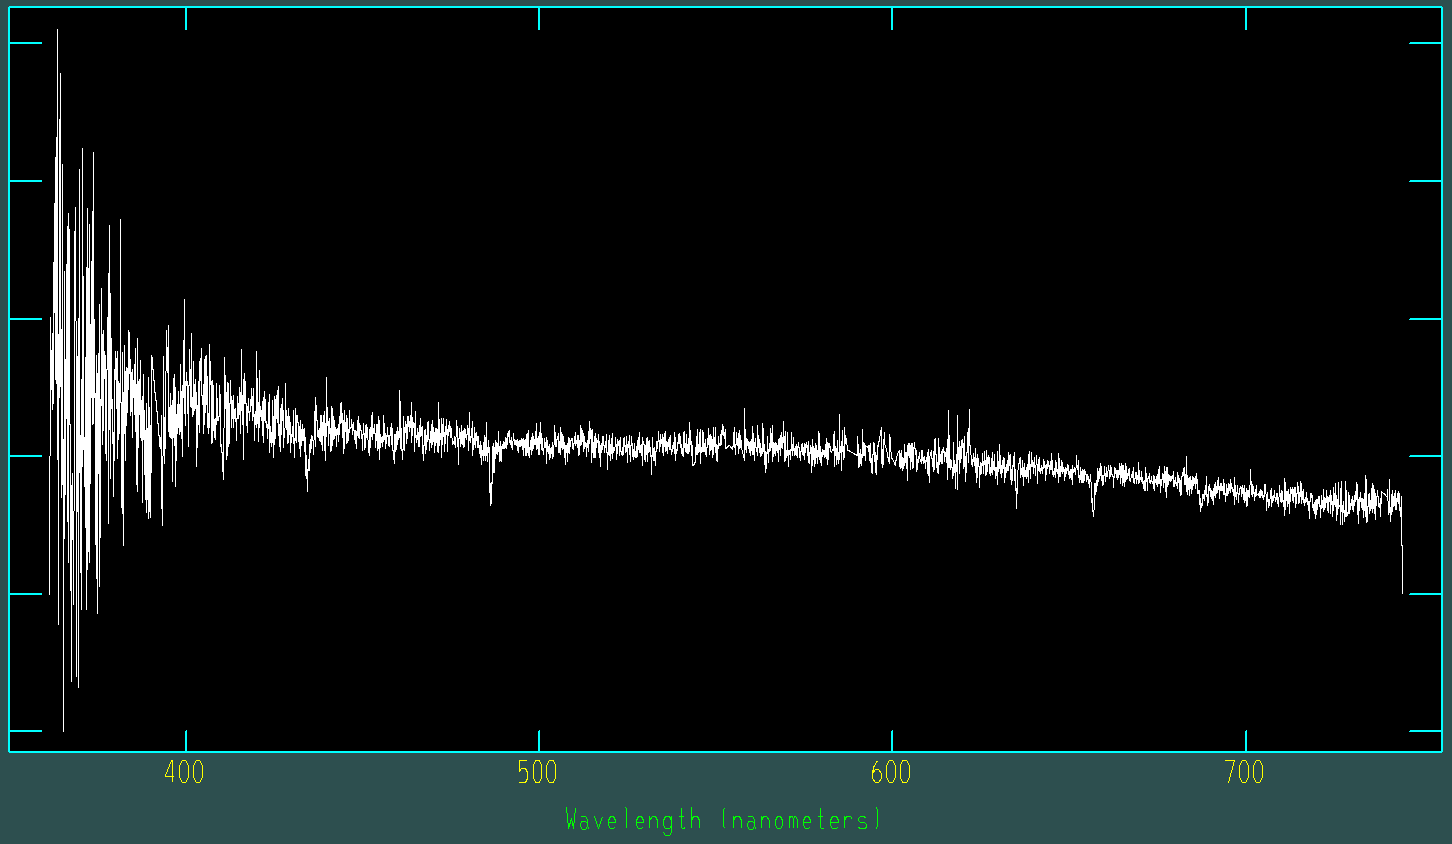
\includegraphics[width=\textwidth]{proposatal_candidatas_1/UCG02.png}
        \caption{UCG02}
    \end{subfigure}
    \begin{subfigure}[b]{0.22\textwidth}
        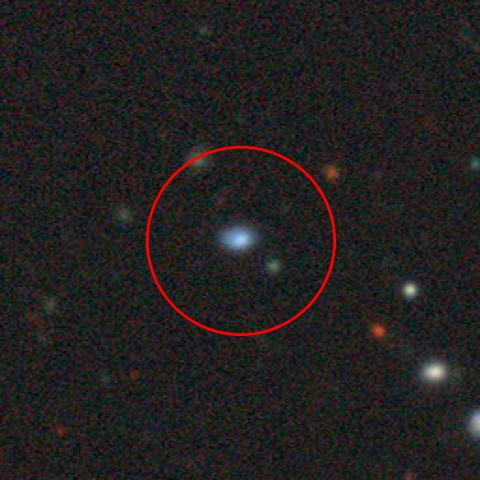
\includegraphics[width=\textwidth]{proposatal_candidatas_1/UCG03.jpg}
        \caption{UCG03}
    \end{subfigure}
    \begin{subfigure}[b]{0.22\textwidth}
        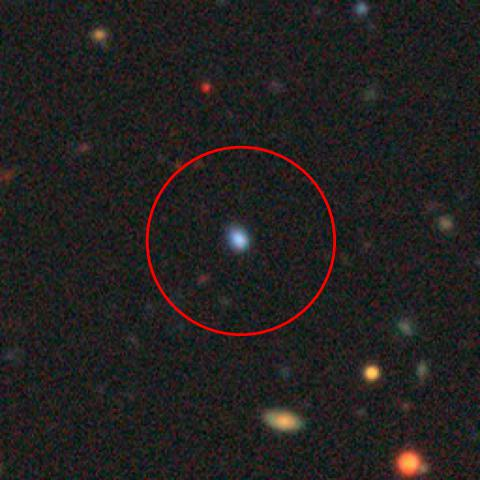
\includegraphics[width=\textwidth]{proposatal_candidatas_1/UCG04.jpg}
        \caption{UCG04}
    \end{subfigure}
    \begin{subfigure}[b]{0.22\textwidth}
        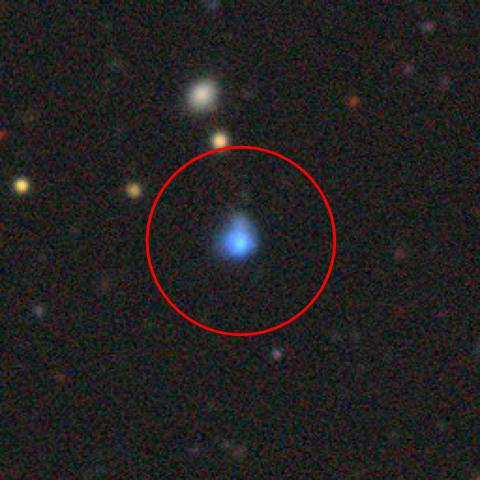
\includegraphics[width=\textwidth]{proposatal_candidatas_1/UCG05.jpg}
        \caption{UCG05}
    \end{subfigure}
    \begin{subfigure}[b]{0.22\textwidth}
        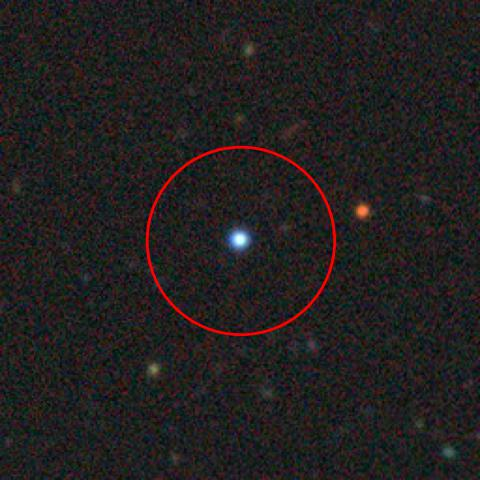
\includegraphics[width=\textwidth]{proposatal_candidatas_1/UCG06.jpg}
        \caption{UCG06}
    \end{subfigure}
    \begin{subfigure}[b]{0.22\textwidth}
        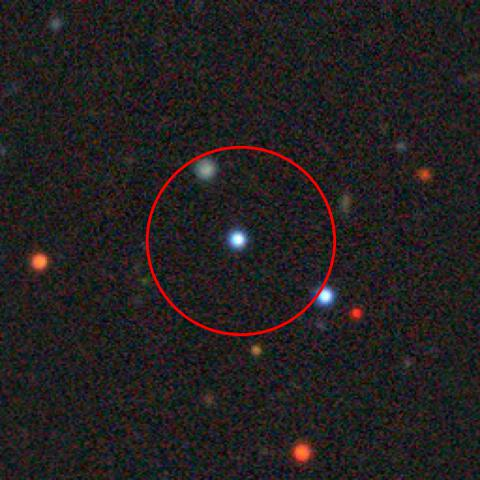
\includegraphics[width=\textwidth]{proposatal_candidatas_1/UCG07.jpg}
        \caption{UCG07}
    \end{subfigure}
    \begin{subfigure}[b]{0.22\textwidth}
        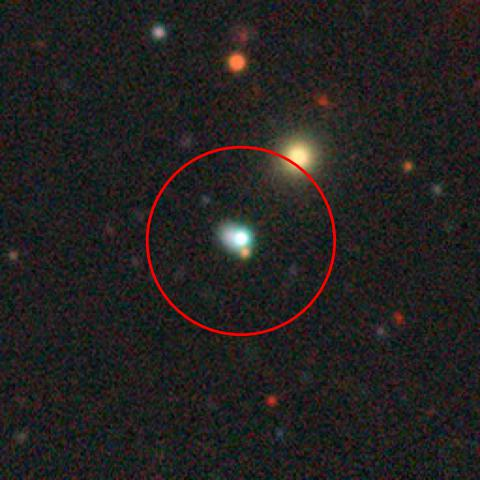
\includegraphics[width=\textwidth]{proposatal_candidatas_1/UCG08.jpg}
        \caption{UCG08}
    \end{subfigure}
    \begin{subfigure}[b]{0.22\textwidth}
        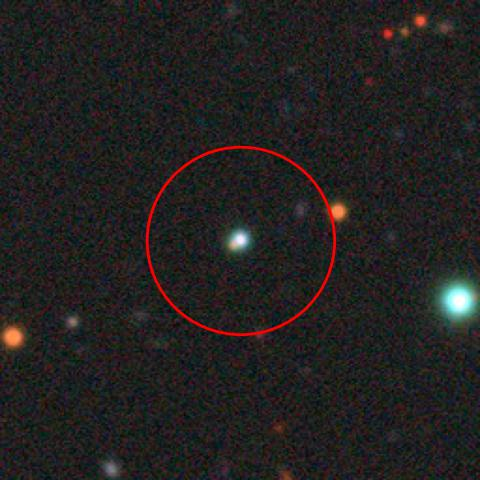
\includegraphics[width=\textwidth]{proposatal_candidatas_1/UCG09.jpg}
        \caption{UCG09}
    \end{subfigure}
    \begin{subfigure}[b]{0.22\textwidth}
        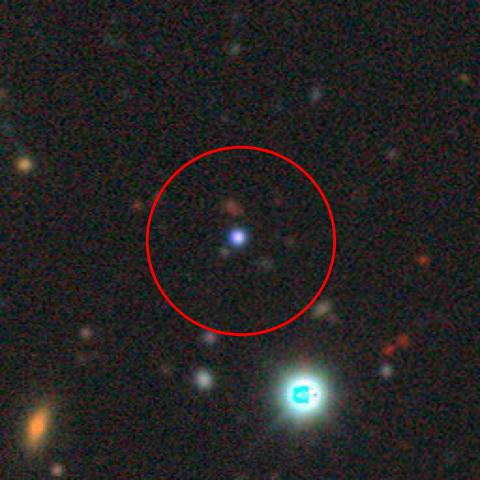
\includegraphics[width=\textwidth]{proposatal_candidatas_1/UCG10.jpg}
        \caption{UCG10}
    \end{subfigure}
    \begin{subfigure}[b]{0.22\textwidth}
        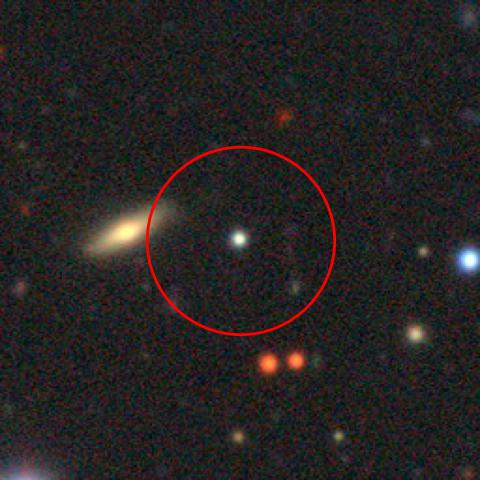
\includegraphics[width=\textwidth]{proposatal_candidatas_1/UCG11.jpg}
        \caption{UCG11}
    \end{subfigure}
    \begin{subfigure}[b]{0.22\textwidth}
        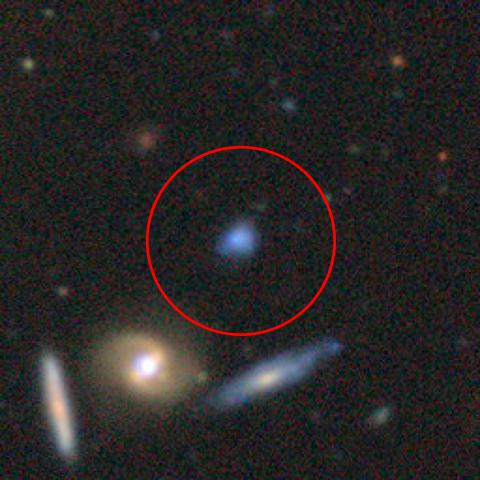
\includegraphics[width=\textwidth]{proposatal_candidatas_1/UCG12.jpg}
        \caption{UCG12}
    \end{subfigure}
    \begin{subfigure}[b]{0.22\textwidth}
        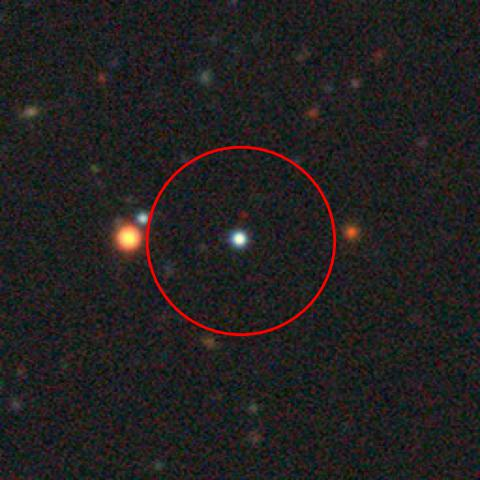
\includegraphics[width=\textwidth]{proposatal_candidatas_1/UCG13.jpg}
        \caption{UCG13}
    \end{subfigure}
    \begin{subfigure}[b]{0.22\textwidth}
        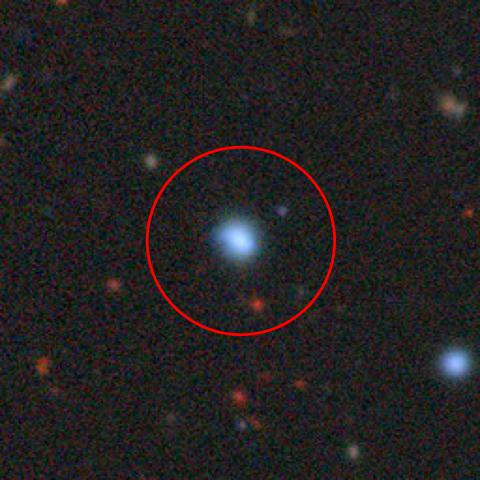
\includegraphics[width=\textwidth]{proposatal_candidatas_1/UCG14.jpg}
        \caption{UCG14}
    \end{subfigure}
    \begin{subfigure}[b]{0.22\textwidth}
        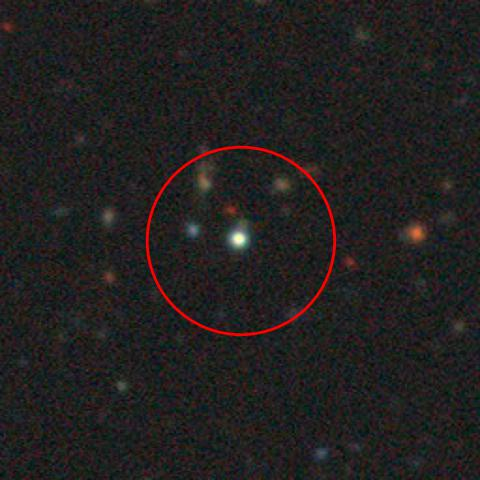
\includegraphics[width=\textwidth]{proposatal_candidatas_1/UCG15.jpg}
        \caption{UCG15}
    \end{subfigure}
    \begin{subfigure}[b]{0.22\textwidth}
        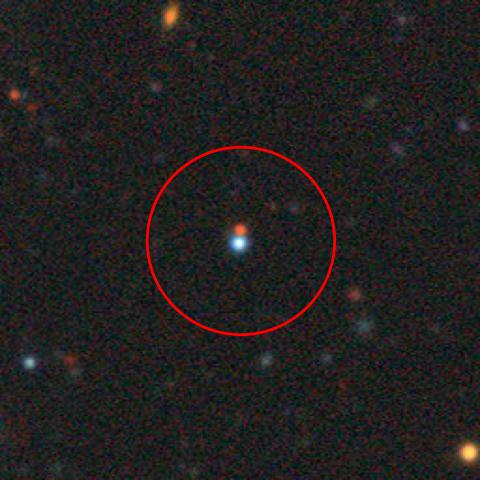
\includegraphics[width=\textwidth]{proposatal_candidatas_1/UCG16.jpg}
        \caption{UCG16}
    \end{subfigure}
    \begin{subfigure}[b]{0.22\textwidth}
        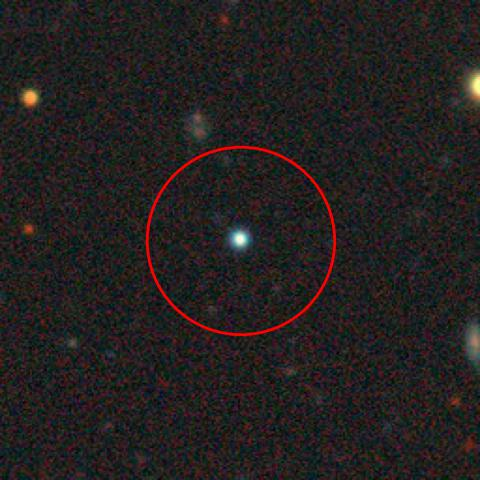
\includegraphics[width=\textwidth]{proposatal_candidatas_1/UCG17.jpg}
        \caption{UCG17}
    \end{subfigure}
    \begin{subfigure}[b]{0.22\textwidth}
        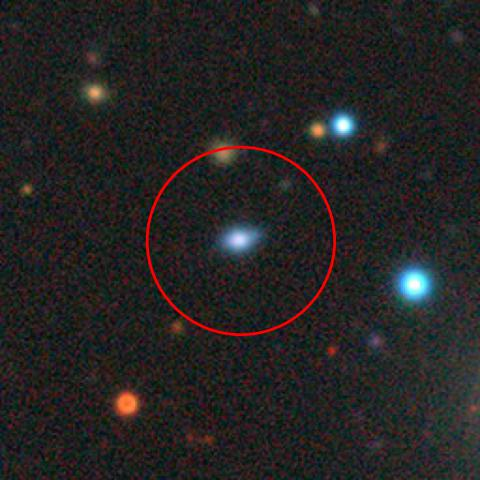
\includegraphics[width=\textwidth]{proposatal_candidatas_1/UCG18.jpg}
        \caption{UCG18}
    \end{subfigure}
    \caption{Imagens das candidatas do conjunto de candidatas a UCDs observadas com o GMOS no telescópio Gemini Sul selecionadas de um projeto anterior. Imagens obtidas pelo Legacy Survey. Os nomes correspondem ao mesmo nome do objeto da tabela \ref{candidatas_espectroscopia_1}.}
    \label{candidatas_espectroscopia_1_img}
\end{figure}


\vspace{\baselineskip}


\subsection*{Candidatas com sinais de linhas de emisssão}
A partir da lista de candidatas explicadas na sessão \ref{cap:selecao_candidatas}, com 7081 objetos, selecionamos algumas com características interessantes para um pedido de tempo de espectroscopia. Utilizando a ferramenta Astroinspect \cite{astroinspect}, podemos fornecer uma tabela de objetos, e ela nos retorna, por exemplo, o \textit{Photo Spec}, isto é, uma imagem do espectro do objeto a partir das medições dos filtros fotométricos do S-PLUS.

\vspace{\baselineskip}

Nosso objetivo inicial foi, dentro dessa amostra de candidatas, encontrar aquelas cujo \textit{Photo Spec} apresentassem um salto nas medições do filtro J0660. Esse salto poderia indicar a presença de linhas de emissão de Halpha (esperados para esse filtro em repouso), o que seria um indicativo de que, dado o redshift baixo de Fornax, poderíamos estar observando objetos dentro do intervalo de redshifts compatíveis com o aglomerado. Isso é, se existir algum objeto com emissões em Halpha em Fornax, é esperado ser observado um salto no filtro J0660, mesmo que levemente deslocado em relação ao filtro em repouso.

\vspace{\baselineskip}

Dos 7081 objetos, selecionamos 6 objetos com sinais de linhas de emissão. Na Figura \ref{photo_spec_candidatas} apresentamos os \textit{Photo Spec} desses objetos, criados com a ferramenta Astroinspect.


\begin{figure}[!ht]
    \centering
    \captionsetup{justification=centering}
    \begin{subfigure}[b]{0.3\textwidth}
        \includegraphics[width=\textwidth]{photo_specs/Candidate_1.png}
        \caption{Candidate\_1}
    \end{subfigure}
    \begin{subfigure}[b]{0.3\textwidth}
        \includegraphics[width=\textwidth]{photo_specs/Candidate_2.png}
        \caption{Candidate\_2}
    \end{subfigure}
    \begin{subfigure}[b]{0.3\textwidth}
        \includegraphics[width=\textwidth]{photo_specs/Candidate_3.png}
        \caption{Candidate\_3}
    \end{subfigure}
    \begin{subfigure}[b]{0.3\textwidth}
        \includegraphics[width=\textwidth]{photo_specs/Candidate_4.png}
        \caption{Candidate\_4}
    \end{subfigure}
    \begin{subfigure}[b]{0.3\textwidth}
        \includegraphics[width=\textwidth]{photo_specs/Candidate_5.png}
        \caption{Candidate\_5}
    \end{subfigure}
    \begin{subfigure}[b]{0.3\textwidth}
        \includegraphics[width=\textwidth]{photo_specs/Candidate_6.png}
        \caption{Candidate\_6}
    \end{subfigure}
    \caption{Imagens dos \textit{Photo Spec}, criadas pela Ferramenta Astroinspect \cite{astroinspect}, das candidatas a objetos compactos com sinais de linhas de emissão no filtro J0660. Os nomes correspondem ao nome interno usado para o pedido de tempo de observação espectroscópica no Gemini.}
    \label{photo_spec_candidatas}
\end{figure}


Observamos na Figura \ref{photo_spec_candidatas} que os objetos apresentam os sinais de linhas de emissão no filtro J0660, assim como o comentado. Dessa forma, esses objetos foram selecionados para a observação espectroscópica no Gemini Sul. Na figura \ref{candidatas_espectroscopia_2_img} apresentamos as imagens desses objetos.

\begin{figure}[!ht]
    \centering
    \captionsetup{justification=centering}
    \begin{subfigure}[b]{0.25\textwidth}
        \includegraphics[width=\textwidth]{proposatal_candidatas_2/Candidate_1.png}
        \caption{Candidate\_1}
    \end{subfigure}
    \begin{subfigure}[b]{0.25\textwidth}
        \includegraphics[width=\textwidth]{proposatal_candidatas_2/Candidate_2.png}
        \caption{Candidate\_2}
    \end{subfigure}
    \begin{subfigure}[b]{0.25\textwidth}
        \includegraphics[width=\textwidth]{proposatal_candidatas_2/Candidate_3.png}
        \caption{Candidate\_3}
    \end{subfigure}
    \begin{subfigure}[b]{0.25\textwidth}
        \includegraphics[width=\textwidth]{proposatal_candidatas_2/Candidate_4.png}
        \caption{Candidate\_4}
    \end{subfigure}
    \begin{subfigure}[b]{0.25\textwidth}
        \includegraphics[width=\textwidth]{proposatal_candidatas_2/Candidate_5.png}
        \caption{Candidate\_5}
    \end{subfigure}
    \begin{subfigure}[b]{0.25\textwidth}
        \includegraphics[width=\textwidth]{proposatal_candidatas_2/Candidate_6.png}
        \caption{Candidate\_6}
    \end{subfigure}
    \caption{Imagens das candidatas do conjunto de candidatas a objetos compactos com sinais de linhas de emissão no filtro J0660. Imagens obtidas pelo Legacy Survey. Os objetos correspondem com a mesma lista de \textit{Photo Spec} da Figura \ref{photo_spec_candidatas}.}
    \label{candidatas_espectroscopia_2_img}
\end{figure}

\section{Redução dos Espectros}
Os dados espectroscópicos do telescópio Gemini não passam por um tratamento inicial, então é necessário um pré-processamento. Esse passo é crucial para limpar as imagens de sinais indesejados, removendo ruídos dos instrumentos e convertendo os espectros bidimensionais em unidimensionais para análise.

Fizemos a redução dos dados usando o Software de Redução de Dados DRAGONS (Data Reduction for Astronomy with Gemini Observatory's Node System) \cite{dragons_python}. Esse software permite reduzir os dados tanto pela linha de comando quanto por meio de uma API em Python. Optamos pela API em Python para tornar o processo mais eficiente e agilizar a geração dos espectros unidimensionais (1D) e bidimensionais (2D) para cada objeto.

\subsection*{Seleção de~Dados}

O primeiro passo para a redução é a seleção dos dados que serão usados, como os arquivos de \textit{bias}, \textit{flats}, \textit{arcs}, estrelas padrão (\textit{standard star}) e os dados científicos. Utilizamos a função \verb|dataselect.select_data|, que permite filtrar os arquivos por algumas características específicas, como o tipo de detector e o objeto observado.

\subsection*{Redução do \textit{Bias}}

A etapa inicial da redução é a correção de \textit{bias}, onde os arquivos são processados para remover o sinal eletrônico residual presente nas imagens. Utilizando a função \verb|Reduce|, criamos dois conjuntos de arquivos de \textit{bias}: um para as estrelas padrão e outro para os dados científicos. Essa correção visa garantir que o sinal obtido nas observações não seja contaminado por ruídos instrumentais.

\subsection*{Redução dos \textit{Flats}}

Após a correção de \textit{bias}, processamos as imagens de \textit{flat-field}, que corrigem variações na resposta do detector em diferentes regiões do campo de visão. Os arquivos de \textit{flats} são selecionados e processados novamente com a função \verb|Reduce|, assegurando a uniformidade na resposta do detector em todas as partes do espectro.

\subsection*{Redução dos \textit{Arcs}}

Na sequência, realizamos a redução dos arquivos de \textit{arcs}, que contêm linhas de emissão conhecidas utilizadas para calibrar a escala de comprimento de onda dos espectros. A função \verb|Reduce| é aplicada para processar os \textit{arcs}, ajustando as linhas de emissão observadas ao modelo teórico e garantindo que os comprimentos de onda sejam medidos com precisão.

\subsection*{Redução da Estrela Padrão}

Para a redução da estrela padrão (\textit{standard star}), também utilizamos a função \verb|Reduce| para processar essas observações, gerando um espectro calibrado em fluxo, que serve como referência para a normalização dos espectros dos objetos científicos. O espectro resultante é plotado e analisado para verificar a qualidade da calibração.

\subsection*{Redução dos Dados Científicos}

Finalmente, os dados científicos são reduzidos aplicando todas as correções anteriores (\textit{bias}, \textit{flat}, \textit{arc}) aos dados de observação dos objetos de interesse, novamente utilizando a função \verb|Reduce|. Esse processo resulta na geração dos espectros unidimensionais (\textit{1D}) e bidimensionais (\textit{2D}) que poderão ser analisados.

\section{Análise dos Espectros}

\section{Análise dos espectros das candidatas}


